\documentclass{scrreprt}
\usepackage[utf8]{inputenc}
\usepackage{xcolor}
\usepackage{amsmath,amsthm,amssymb,amsfonts, fancyhdr, color, comment, graphicx, environ}
\usepackage[explicit]{titlesec}
\usepackage{soul}
\usepackage[top=1.8cm, bottom=2cm, left=1.5cm, right=1.5cm]{geometry}
\usepackage{karnaugh-map}
\usepackage{booktabs}
\usepackage{mdframed}
\usepackage{fix-cm}
\usepackage{tabularx}
\usepackage{tikz, fouriernc}
\usetikzlibrary{calc}
\usepackage[hidelinks]{hyperref}
\usepackage[spanish]{babel}
\usepackage[backend=biber]{biblatex}
\bibliography{refs.bib}

\usepackage[many]{tcolorbox}    	% for COLORED BOXES (tikz and xcolor included)

\newtcolorbox{codebox}[2][]{
    sharpish corners, % better drop shadow
    boxrule = 0pt,
    toprule = 4.5pt, % top rule weight
    enhanced,
    enlarge top by=5pt,
    colback = white,
    before skip = 0.2cm,    % add extra space before the box
    after skip = 0.5cm,      % add extra space after the box
    drop fuzzy shadow = black!35,
    fontupper=\footnotesize\sffamily,
    fonttitle=\footnotesize\sffamily\color{black},
    title=#2,
    attach boxed title to bottom right={xshift=6pt,yshift=6pt},
    boxed title style={
        enhanced,
        arc=0pt,
        outer arc=0pt,
        boxrule = 0pt,
        colback = white,
        drop fuzzy shadow = black!35,
    },
    #1,
}

\usepackage{listings}

\newcounter{pascalcode}[section]

\renewcommand{\thepascalcode}{\arabic{section}.\arabic{pascalcode}}

\lstdefinelanguage{pascal-like}{
  morekeywords={var, type, spec, destroy, constructors, operations, tuple, enumerate, fi, ret, downto, where, proc, fun, in, out, if, then, else, while, do, for, to, end, od},
  morecomment=[s]{\{-}{-\}},
  morestring=[b]",
  sensitive=true,
  keywordstyle=\color{orange},
  commentstyle=\color{green!70!black},
  stringstyle=\color{blue!70!black},
  %numbers=left,
  %numberstyle=\tiny\color{gray},
  alsoletter={:,=,+,-,*,>,<,(,)},
  morekeywords=[2]{:,=,+,-,*,>,<,(,),&,&&,||,!,!=,==},
  keywordstyle=[2]{\color{blue}},
  literate={:=}{{\textcolor{green!50!black}{:=}}}2,
  morekeywords=[3]{nat, array, of, int, real, bool, char}, 
  keywordstyle=[3]{\color{blue!40!black}},
  mathescape=true
}

\lstnewenvironment{pascallike}[1][]{
  \refstepcounter{pascalcode}
  \lstset{
    language=pascal-like,
    %numbers=left,
    %numberstyle=\tiny\color{gray},
    %captionpos=b,
    #1
  }
}{\phantomsection\addcontentsline{lol}{section}{Código \thepascalcode}}

\definecolor{lime}{RGB}{0,0,128}
\definecolor{titleblue}{HTML}{4a7aa4}
\setlength{\parindent}{0pt}

\pagestyle{fancy}
\fancyhf{} % Limpia los encabezados y pies de página existentes
\lhead{Villar Pedro} % Añade "Nombre" al lado izquierdo del encabezado
\rhead{\leftmark} % Añade la sección actual al lado derecho del encabezado

\newtcolorbox{titlecolorbox}[1]{ %the box around chapter
    coltext=white,
    colframe=black,
    colback=black,
    boxrule=0pt,
    arc=0pt,
    notitle,
    width=4.8em,
    height=2.4ex,
    before=\hfill
}

\usepackage{xcolor}

\renewcommand{\chaptername}{Capítulo}
\titlespacing*{\chapter}{0pt}{0pt}{0pt}
\titleformat{\chapter}[display]
  {\sffamily\Huge}
  {}
  {0pt}
  {\begin{titlecolorbox}{}
  {\large\sffamily\MakeUppercase{\chaptername}}
  \end{titlecolorbox}
  \vspace*{-4.19ex}\noindent\rule{\textwidth}{0.4pt}
  \parbox[b]{\dimexpr\textwidth-4.8em\relax}{\raggedright\MakeUppercase{#1}}{\hfill\fontsize{70}{60}\selectfont\thechapter}
  }
  []

\titleformat{name=\chapter,numberless}[display]
  {\sffamily\Huge}
  {}
  {0pt}
  {\begin{titlecolorbox}{}
  {\large\sffamily\MakeUppercase{\chaptername}}
  \end{titlecolorbox}
  \vspace*{-4.19ex}\noindent\rule{\textwidth}{0.4pt}
  \parbox[b]{\dimexpr\textwidth-4.8em\relax}{\raggedright\MakeUppercase{#1}}
  }
  []

\titleformat{\section}[display]
  {\sffamily\large}
  {}
  {0pt}
  {\hrule\vspace*{0.25ex}\parbox[b]{\dimexpr\textwidth\relax}{\textcolor{darkgray}{\thesection}\quad\raggedright\bfseries\MakeUppercase{#1}}}
  [\hrule]

\titleformat{\subsection}[display]
  {\sffamily\large}
  {}
  {0pt}
  {\parbox[b]{\dimexpr\textwidth\relax}{\textcolor{darkgray}{\thesubsection}\quad\raggedright\bfseries{#1}}}
  []

\titleformat{\subsubsection}[display]
  {\sffamily\large}
  {}
  {0pt}
  {\parbox[b]{\dimexpr\textwidth\relax}{\textcolor{darkgray}{\thesubsubsection}\quad\raggedright\bfseries{#1}}}
  []
  
\bibliography{refs.bib}

\begin{document}
\begin{titlepage}
    \begin{tikzpicture}[overlay,remember picture]
        \fill[lime!10] (current page.south east) rectangle (current page.north west);
        \fill[lime,even odd rule] (current page.south west) rectangle ([xshift=1.5cm]current page.north west) ($(current page.north west)!.5!(current page.south west)$) arc(180:270:3) ($(current page.north west)!.5!(current page.south west)$) arc(270:450:3.5) ([yshift=7cm]$(current page.north west)!.5!(current page.south west)$)  arc(180:90:3);
  %           \draw[lime!10,double=lime!10,double distance=2mm] (current page.south west) --+ (2,2) --+ (-2,6) --+ (2,8) --+ (-2,9) --+ (2,13) --+ (-2,18) --+ (2,30);
            \draw[lime,thin] (13,-1) node[lime,above left] {\Huge Algoritmos 2 - TP} --+ (0,3) node[lime,below right] {\Huge 1C-2024};
        \node[yshift=-5cm,xslant=1,yscale=1.6,lime!40,opacity=.2] at (9.5,-6.5) {\scalebox{6}{Apunte}};
        \node[yshift=-5cm,lime] at (8,-7) {\scalebox{6}{Apunte}};
            \draw[lime,fill=titleblue!20] ([xshift=-1cm]current page.north east) -- ([yshift=-1cm]current page.north east) -- ([yshift=-2cm]current page.north east) -- ([xshift=-2cm]current page.north east);
        \path ([xshift=-1cm]current page.north east) -- ([yshift=-1cm]current page.north east) node[midway,sloped,below=.1cm,lime] {Villar Pedro};
    \end{tikzpicture}
  \end{titlepage}
\tableofcontents
\chapter{Introducción al lenguaje de programación de la materia}

El lenguaje a utilizar está inspirado en el lenguaje imperativo \textit{Pascal}, al cual se le han ido realizando modificaciones de acuerdo a las necesidades didácticas de la materia. Se utilizará principalmente para la incorporación de conceptos tales como análisis de algoritmos, definición de tipos abstractos de datos, o la comprensión de distintas técnicas de programación. 

\section{Tipos de datos}
En este lenguaje, existen varios tipos de datos, incluyendo:
\begin{itemize}
    \item \texttt{int}: para valores enteros,
    \item \texttt{real}: para valores decimales,
    \item \texttt{bool}: para valores de verdad (verdadero o falso),
    \item \texttt{char}: para caracteres.
\end{itemize}
Además, se pueden crear estructuras de datos más complejas como arreglos para agrupar elementos del mismo tipo.

\subsection{Declaración de variables}
Las variables se declaran utilizando la palabra clave \texttt{var}, seguida de una lista de variables separadas por comas. Cada variable debe tener un tipo asociado. Por ejemplo:

\begin{codebox}{Código 1}
\footnotesize Declaración de variables
\tcblower
\begin{pascallike}
    {- Variable entera -}
    var i : int
    i := 10
    {- Variable real -}
    var x : real
    x := 3.14
    {- Variable booleana -}
    var b : bool
    b := true
    {- Variable caracter -}
    var c : char
    c := 'a'
\end{pascallike}
\end{codebox}

\section{Operadores}
Los operadores aritméticos básicos son \texttt{+}, \texttt{-}, \texttt{*} y \texttt{/}. Además, se pueden utilizar los operadores de comparación \texttt{<}, \texttt{>}, \texttt{<=}, \texttt{>=}, \texttt{==} y \texttt{!=}.
\begin{codebox}{Código 2}
\footnotesize Uso de operadores
\tcblower
\begin{pascallike}
    {- Operadores aritmeticos -}
    var a : int
    a := 10 + 5
    a := 10 - 5
    a := 10 * 5
    a := 10 / 5
    {- Operadores de comparacion -}
    var b : bool
    b := 10 < 5
    b := 10 > 5
    b := 10 <= 5
    b := 10 >= 5
    b := 10 == 5
    b := 10 != 5
\end{pascallike}
\end{codebox}
Junto con las constantes lógicas \texttt{true} y \texttt{false}, se pueden utilizar los operadores lógicos \texttt{\&\&}, \texttt{||} y \texttt{!}.
\begin{codebox}{Código 3}
\footnotesize Uso de operadores lógicos
\tcblower
\begin{pascallike}
    {- Operadores logicos -}
    var b : bool
    b := true && false
    b := true || false
    b := !true
\end{pascallike}
\end{codebox}
\textbf{No hay operadores definidos para el tipo \texttt{char}.}

\section{Tipos de datos estructurados}
Un tipo estructurado permite representar colecciones de otros tipos de datos. De manera similar a los tipos básicos, se definen operaciones específicas para acceder a los elementos que conforman al tipo. En el lenguaje solo tenemos definidos de forma nativa a los arreglos.

Para definir un arreglo es necesario detallar el tipo de sus componentes y los tamaños para cada una de sus dimensiones, los cuales deberán ser mayores a cero.

\begin{codebox}{Código 4}
\footnotesize Declaración de arreglos
\tcblower
\begin{pascallike}
    {- Arreglo de enteros -}
    var a : array [1..10] of int
    a[1] := 10
    {- Arreglo de reales -}
    var b : array [1..10] of real
    b[1] := 3.14
    {- Arreglo de booleanos -}
    var c : array [1..10] of bool
    c[1] := true
    {- Arreglo de caracteres -}
    var d : array [1..10] of char
    d[1] := 'a'
\end{pascallike}
\end{codebox}
En este ejemplo, se declaran arreglos de 10 elementos de distintos tipos. Luego, se asigna un valor a la primera posición de cada arreglo.

\section{Definición de tipos}
El lenguaje permite definir tipos de datos personalizados. Esto es útil para abstraer la representación de un concepto y facilitar la comprensión del código. Por ejemplo, se puede definir un tipo \texttt{punto} para representar un punto en el plano cartesiano.

\begin{codebox}{Código 5}
\footnotesize Definición de tipos
\tcblower
\begin{pascallike}
type punto = tuple
                x : real
                y : real
                end tuple
\end{pascallike}
\end{codebox}
En este ejemplo, se define un tipo \texttt{punto} que contiene dos campos \texttt{x} e \texttt{y} de tipo \texttt{real}. Luego, se pueden declarar variables de tipo \texttt{punto} y asignarles valores.
\section{Tipos enumerados}
Un tipo enumerado representa un conjunto finito de valores. Cada valor está definido mediante un identificador único. Para declarar un tipo enumerado se emplean las palabras claves \textbf{enumerate} y \textbf{end enumerate}. Por ejemplo, definamos un tipo enumerado para los días de la semana.

\begin{codebox}{Código 6}
\footnotesize Definición de tipos enumerados
\tcblower
\begin{pascallike}
type day = enumerate
            Lunes
            Martes
            Miercoles
            Jueves
            Viernes
            Sabado
            Domingo
            end enumerate
\end{pascallike}
\end{codebox}
Ya una vez definido el tipo enumerado, se pueden declarar variables de este tipo y asignarles valores.

\begin{codebox}{Código 7}
\footnotesize Uso de tipos enumerados
\tcblower
\begin{pascallike}
var d : day
d := Lunes
\end{pascallike}
\end{codebox}

\section{Sinónimos de tipos}
Un sinónimo de tipo es una forma de referirse a un tipo de datos con un nombre diferente. Por ejemplo, se puede definir un sinónimo de tipo \texttt{real} para representar la temperatura en grados Celsius.

\begin{codebox}{Código 8}
\footnotesize Definición de sinónimos de tipos
\tcblower
\begin{pascallike}
type celsius = real
\end{pascallike}
\end{codebox}
No necesariamente los sinónimos de tipo deben ser de tipos básicos, también se pueden definir sinónimos de tipos estructurados.

\begin{codebox}{Código 9}
\footnotesize Definición de sinónimos de tipos estructurados
\tcblower
\begin{pascallike}
type matrizdereales = array [1..10] of real
\end{pascallike}
\end{codebox}

Una expresión de este tipo, es útil cuando se utiliza una función donde se espera un valor de uno de los sinónimos de su tipo. En el siguiente ejemplo se declara una variable \texttt{mR} del tipo \texttt{matrizdereales}, y se opera de manera transparente como si fuese un arreglo tradicional.

\begin{codebox}{Código 10}
\footnotesize Uso de sinónimos de tipos
\tcblower
\begin{pascallike}
var mR : matrizdereales
for i := 0 to 9 do
    for j := 0 to 9 do
        mR[i, j] := 0.0
    od
od
\end{pascallike}
\end{codebox}

\section{Tuplas}
Una tupla es un tipo de dato estructurado que permite agrupar un número finito de elementos de distintos tipos. Para definir una tupla se emplean las palabras claves \textbf{tuple} y \textbf{end tuple}. Por ejemplo, definamos una tupla para representar los datos de una persona.

\begin{codebox}{Código 11}
\footnotesize Definición de tuplas
\tcblower
\begin{pascallike}
type persona = tuple
                nombre : string
                edad : int
                altura : real
                end tuple
\end{pascallike}
\end{codebox}
Y para darle valor a una variable de tipo \texttt{persona} se hace de la siguiente manera.

\begin{codebox}{Código 12}
\footnotesize Uso de tuplas
\tcblower
\begin{pascallike}
var p : persona
p.nombre := "Juan"
p.edad := 20
p.altura := 1.80
\end{pascallike}
\end{codebox}

\section{Funciones y procedimientos}
Las funciones y procedimientos son bloques de código que pueden ser invocados desde otros bloques de código. La diferencia entre ambos radica en que las funciones devuelven un valor, mientras que los procedimientos no. La sintaxis para definir funciones y procedimientos es la siguiente:

\begin{codebox}{Código 13}
\footnotesize Definición de funciones 
\tcblower
\begin{pascallike}
fun nombre (p1 : T1, p2 : T2, ... , pn : Tn) ret r : T
    {- Cuerpo de la funcion -}
end fun 
\end{pascallike}
\end{codebox}
Esta función toma los parametros \texttt{p1}, \texttt{p2}, ..., \texttt{pn} de tipos \texttt{T1}, \texttt{T2}, ..., \texttt{Tn} respectivamente, y devuelve un valor de tipo \texttt{T}. Por ejemplo, definamos una función que sume dos números enteros.

\begin{codebox}{Código 14}
\footnotesize Función suma
\tcblower
\begin{pascallike}
fun suma (a : int, b : int) ret r : int
    ret := a + b
end fun
\end{pascallike}
\end{codebox}

En el siguiente ejemplo se muestra la implementación de la función \texttt{factorial}, que calcula el factorial de un número entero positivo \texttt{n}. La variable de retorno fact almacena la productoria de números, y al finalizar la ejecución de la función, se retorna su valor al contexto donde se efectuó la llamada. El comentario simplemente indica la precondición ha satisfacer para garantizar el comportamiento esperado de la función.

\begin{codebox}{Código 15}
\footnotesize Función factorial
\tcblower
\begin{pascallike}
{- PRE : n >= 0 -}
fun factorial (n : int) ret fact : int
    fact := 1
    for i := 2 to n do
        fact := fact * i
    od
end fun
\end{pascallike}
\end{codebox}

Un procedimiento realiza una computación de acuerdo a un conjunto de parámetros de lectura, para modificar un conjunto de parámetros de escritura. Su comportamiento es determinado solamente por los parámetros que recibe donde cada uno lleva un decorado que indica si es de lectura \texttt{in}, de escritura \texttt{out}, o ambas \texttt{in/out}. Un procedimiento no modifica el estado de los parámetros de lectura, y tampoco consulta el estado de los parámetros de escritura.

En el siguiente ejemplo se implementa el procedimiento initialize, el cual se encarga de inicializar un arreglo de enteros según un valor determinado. Lo interesante a destacar en este ejemplo es la forma en que se manejan los parámetros de lectura y escritura. El parámetro de lectura solo ocurre del lado derecho de la asignación, mientras que el parámetro de escritura solo ocurre del lado izquierdo. Esto significa que al llamar a la función initialize, se pasarán los parámetros como argumentos de lectura (para ser utilizados dentro de la función) y como argumentos de escritura (para almacenar el resultado de la función).

\begin{codebox}{Código 16}
\footnotesize Procedimiento initialize
\tcblower
\begin{pascallike}
proc initialize ( in e : int , out a : array [ 10 ] of int )
    for i := 9 downto 0 do
        a [ i ] := e
    od
end proc
\end{pascallike}
\end{codebox}

\section{Recursión}
El lenguaje soporta la recursión, es decir, una función o procedimiento puede llamarse a sí mismo. Por ejemplo, definamos una función que calcule el factorial de un número de manera recursiva. Por ejemplo definamos la función factorial de la siguiente manera.

\begin{codebox}{Código 17}
\footnotesize Función factorial recursiva
\tcblower
\begin{pascallike}
{- PRE : n >= 0 -}
fun factorial (n : int) ret fact : int
    if n >= 2 then
        fact := n * factorial(n - 1)
    else
        fact := 1
    fi
end fun
\end{pascallike}
\end{codebox}

\section{Polimorfismo paramétrico}
El lenguaje soporta el polimorfismo paramétrico, es decir, la capacidad de definir funciones y procedimientos que operan sobre un rango de tipos. Por ejemplo, definamos una función que intercambie los valores de dos variables de cualquier tipo.

\begin{codebox}{Código 18}
\footnotesize Función swap
\tcblower
\begin{pascallike}
proc swap ( in / out a : array [ n ] of T , in i , j : int )
    var temp : T
    temp := a[i]
    a[i] := a[j] 
    a[j] := temp
end fun
\end{pascallike}
\end{codebox}

\section{Polimorfismo \textit{Ad Hoc}}
El lenguaje soporta el polimorfismo \textit{Ad Hoc}, es decir, la capacidad de definir funciones y procedimientos que podrían ser implementados de manera genérica pero no para cualquier tipo de datos, sino para ciertos tipos que comparten alguna característica, en consecuencia no es posible utilizar polimorfismo paramétrico.
Consideremos las siguientes implementaciones de \texttt{belongs} y \texttt{selectionSort}. La primera decide si un valor determinado pertenece a un arreglo y la segunda permite ordenar un arreglo de menor a mayor.

\begin{codebox}{Código 19}
\footnotesize Función belongs
\tcblower
\begin{pascallike}
fun belongs ( e : int , a : array [ n ] of int ) ret b : bool
var i : int
i : = 0
b : = false
    while ! b && i < n do
        b : = a [ i ] = = e
        i : = i + 1
    od
end fun    
\end{pascallike}
\end{codebox}

\begin{codebox}{Código 20}
\footnotesize Procedimiento selectionSort
\tcblower
\begin{pascallike}
proc selectionSort ( in / out a : array [ n ] of int )
var minPos : int
    for i : = 0 to n - 1 do
        minPos : = i
        for j : = i + 1 to n - 1 do
            if a [ j ] < a [ minPos ] then minPos : = j fi
        od
        swap ( a , i , minPos )
    od
end proc
\end{pascallike}
\end{codebox}
En ambas implementaciones los elementos son de tipo entero. Sin embargo podríamos definir las mismas operaciones para otros tipos de datos, como por ejemplo, caracteres. Se tendrían que redefinir las anteriores con los nombres \texttt{belongsInt} y \texttt{selectionSortInt}, y declarar de manera idéntica las operaciones \texttt{belongsChar} y \texttt{selectionSortChar} donde solo cambiaríamos int por char en los tipos de los parámetros. Con un trabajo tediosamente repetitivo se podrían dar declaraciones para todos los tipos que tengan definidas las operaciones de comparación; aunque no sería posible para aquellos que no las tengan definidas. El \textit{polimorfismo ad hoc} nos permite escribir de manera genérica una función o un procedimiento donde la tarea que realiza sólo está bien definida para algunos tipos. Además esta tarea puede no ser la misma dependiendo del tipo.

En el lenguaje se definen una serie de clases las cuales pueden ser pensadas como una especie de interfaz que caracteriza algún comportamiento. Un tipo es una instancia de una clase, cuando implementa el comportamiento que la clase describe. El lenguaje sólo incorpora de forma nativa las clases \textbf{Eq} y \textbf{Ord}, y no existe posibilidad de declarar nuevas clases. La primera representa a los tipos que tienen alguna noción de igualdad, y sus operaciones definidas comprenden al \texttt{==} y \texttt{!=}. La segunda representa a los tipos que poseen alguna relación de orden, y sus operaciones definidas comprenden al \texttt{<}, \texttt{<=}, \texttt{>=}, \texttt{>}.

\section{Memoria dinámica}
El lenguaje permite manipular explícitamente la memoria dinámica mediante un tipo de datos especial, que llamaremos puntero. Supongamos que deseamos definir el tipo correspondiente a las listas. Una lista permite representar una colección ordenada de elementos de algún tipo de datos, cuyo tamaño es variable; lo cual significa que su tamaño crece tanto como sea necesario, de acuerdo a la cantidad de elementos almacenados. Todos los tipos presentados hasta el momento utilizan una cantidad fija de memoria, la cual no puede ser modificada en tiempo de ejecución. Recordemos una vez más que los arreglos implementados en el lenguaje tienen un tamaño fijo al momento de la ejecución. En este aspecto el uso de punteros resulta fundamental, ya que permiten reservar y liberar memoria en la medida que sea necesario durante la ejecución del programa.

\subsection{Punteros}
Un puntero es una variable que almacena la dirección de memoria de otra variable. En el lenguaje, los punteros se representan con el tipo \textbf{pointer}, indica el lugar de memoria donde se encuentra almacenado el valor de la variable. La sintaxis para declarar un puntero es la siguiente:

\begin{codebox}{Código 21}
\footnotesize Declaración de punteros
\tcblower
\begin{pascallike}
var p : pointer of int
\end{pascallike}
\end{codebox}

\subsection{Ejemplo}

\begin{codebox}{Código 22}
\footnotesize Ejemplo de uso de punteros
\tcblower
\begin{pascallike}
type node of ( T ) = tuple
                        elem : T ,
                        next : pointer of node of ( T )
                        end tuple

type list of ( T ) = pointer of node of ( T )
\end{pascallike}
\end{codebox}

En el ejemplo anterior se declara una lista enlazada denominada list, la cual se compone de una sucesión de nodos node que se integran por los campos elem de cierto tipo paramétrico T, y next el cual referencia al siguiente nodo en la lista.

\subsection{Operaciones con punteros}
En el lenguaje se definen tres operaciones para manipular punteros. El procedimiento nativo \texttt{alloc} toma una variable de tipo puntero, y le asigna la dirección de un nuevo bloque de memoria, cuyo tamaño estará determinado por el tipo de la variable. El operador \texttt{\#} permite acceder al bloque de memoria apuntado por el puntero. El procedimiento nativo \textbf{free} toma una variable de tipo puntero, y libera el respectivo bloque de memoria referenciado.

Retomando el ejemplo de la lista enlazada, los procedimientos \texttt{empty} y \texttt{addL} son utilizados para construir valores del tipo en cuestión.

\begin{codebox}{Código 23}
\footnotesize Procedimiento empty
\tcblower
\begin{pascallike}
proc empty ( out l : list of ( T ) )
    l : = null
end proc
\end{pascallike}
\end{codebox}

El procedimiento empty construye una lista vacía. La constante null representa un puntero que no referencia un lugar de memoria válido. En el ejemplo, la constante representa una lista que no posee ningín nodo.

\begin{codebox}{Código 24}
\footnotesize Procedimiento addL
\tcblower
\begin{pascallike}
proc addL ( in e : T , in / out l : list of ( T ) )
    var p : pointer of node of ( T )
    alloc ( p )
    p - > elem : = e
    p - > next : = l
    l : = p
end proc
\end{pascallike}
\end{codebox}
\chapter{Ordenación elemental}
Generalmente, se considera que la ordenación de un conjunto de elementos es la disposición de los mismos en un orden determinado. En el caso de los algoritmos de ordenación, se busca que los elementos de un conjunto se encuentren en un orden específico, ya sea ascendente o descendente. En este capítulo se presentan los algoritmos de ordenación más simples, los cuales son útiles para ordenar conjuntos de elementos pequeños.

\begin{figure}[h]
\centering
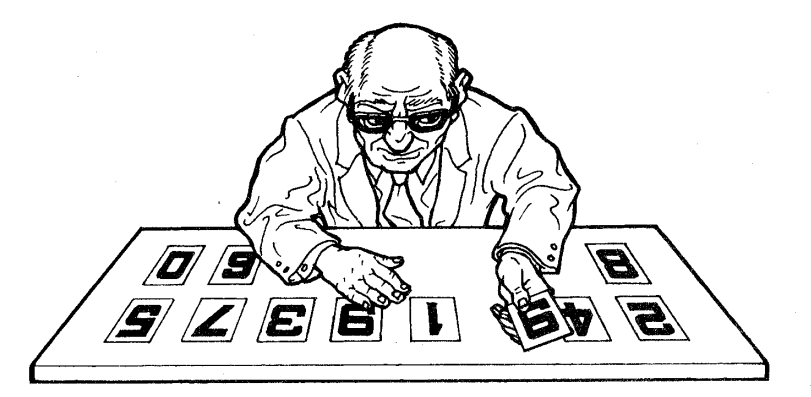
\includegraphics[scale=0.8]{./estáticos/ordenacionArrays.png}
\caption{Ordenación de arreglos}
\end{figure}

La principal condición a imponer a los métodos de ordenación de arreglos es la utilización económica de la memoria disponible. Esto implica que las permutaciones de items, con vistas a su ordenación, deben realizarse utilizando el espacio ocupado por el arreglo y que los métodos que transportan artículos de un array $a$ hacia un array resultado $b$ son intrínsecamente de menor interés.

\section{Ordenación por selección}
Este método se basa en los siguientes principios:
\begin{enumerate}
    \item Seleccionar el menor elemento.
    \item Intercambiarlo con el primer elemento.
\end{enumerate}
Y luego se repite el proceso con el resto del arreglo, es decir, se selecciona el menor elemento del subarreglo restante y se intercambia con el segundo elemento, y así sucesivamente.
\newpage
\begin{figure}[h]
\centering
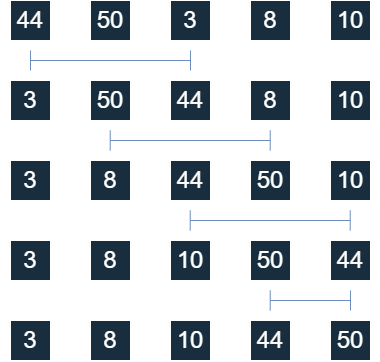
\includegraphics[scale=0.5]{./estáticos/ordSeleccion.png}
\caption{Ejemplo de proceso de ordenación por selección}
\end{figure}

Para el algoritmo de ordenación por selección, se ha desarrollado un procedimiento \texttt{selection\_sort} que recibe un arreglo de tamaño $n$ y lo ordena. El procedimiento \texttt{selection\_sort} utiliza dos funciones auxiliares: \texttt{min\_pos\_from} y \texttt{swap}. La función \texttt{min\_pos\_from} recibe un arreglo y una posición, y retorna la posición del menor elemento a partir de la posición dada. La función \texttt{swap} recibe un arreglo y dos posiciones, e intercambia los elementos en dichas posiciones. Se pueden marcar las siguientes observaciones:

\begin{itemize}
    \item \texttt{selection\_sort} utiliza un ciclo \texttt{for} que recorre el arreglo desde la primera posición hasta la última. En cada iteración, se busca el menor elemento a partir de la posición actual y se intercambia con el elemento en la posición actual,
    \item se encuentra una llamada a la función \texttt{min\_pos\_from} que recibe el arreglo y la posición actual, y retorna la posición del menor elemento a partir de la posición actual,
    \item y se recibe tambien una llamada al procedimiento \texttt{swap} que recibe el arreglo y las posiciones actual y la posición del menor elemento, e intercambia los elementos en dichas posiciones,
    \item encontramos una \textbf{comparación} entre elementos de un arreglo, y una \textbf{asignación} de elementos de un arreglo,
    \item la operación que mas se repite es la comparación de elementos de un arreglo, y toda operación se repite a lo sumo de manera proporcional a esa,
    \item como la celda de un arreglo es constante, su costo no depende de cual es la celda o del tamaño del arreglo, por lo que el costo de la operación es constante.
\end{itemize}

\subsection{Código}

\begin{codebox}{Código 25}
\footnotesize Ordenación por selección
\tcblower
\begin{pascallike}
proc selection_sort (in/out a: array[1..n] of T)
    var minp: nat
    for i := 1 to n do
        minp := min_pos_from(a, i)
        swap(a, i, minp) 
    od
end proc

fun min_pos_from (a: array[1..n] of T, i: nat) ret minp: nat
    minp := i
    for j:= i+1 to n do 
        if a[j] < a[minp] then 
            minp:= j 
        fi
    od
end fun

proc swap (in/out a: array[1..n] of T, in i, j: nat)
    var temp: T
    temp := a[i]
    a[i] := a[j]
    a[j] := temp
end proc
\end{pascallike}
\end{codebox}

\subsection{Análisis de complejidad}
\begin{itemize}
    \item Al llamar a la función \texttt{min\_pos\_from} se realiza una cantidad de operaciones proporcional a $n-i$,
    \item \texttt{selection\_sort} llama a \texttt{min\_pos\_from(a,i)} para $i=1,2,\ldots,n-1$,
    \item por lo tanto, en total son $(n-1) + (n-2) + \ldots + 1 = \frac{n(n-1)}{2}$ comparaciones.
\end{itemize}

\section{Ordenación por inserción}
Este método se basa en los siguientes principios:
\begin{enumerate}
    \item Seleccionar el primer elemento del arreglo.
    \item Insertarlo en la posición correcta.
\end{enumerate}
Y luego se repite el proceso con el resto del arreglo, es decir, se selecciona el siguiente elemento y se inserta en la posición correcta.

\newpage
\begin{figure}[h]
\centering
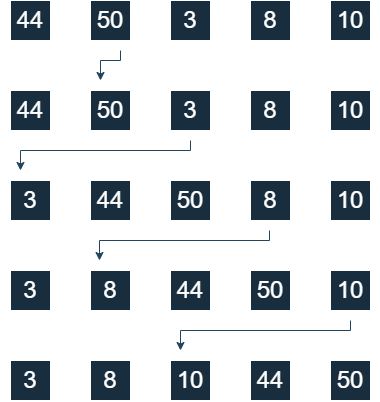
\includegraphics[scale=0.5]{./estáticos/ordInsercion.png}
\caption{Ejemplo de proceso de ordenación por inserción}
\end{figure}

Para el algoritmo de ordenación por inserción, se ha desarrollado un procedimiento \texttt{insertion\_sort} que recibe un arreglo de tamaño $n$ y lo ordena. El procedimiento \texttt{insertion\_sort} utiliza un procedimiento auxiliar \texttt{insert}. El procedimiento \texttt{insert} recibe un arreglo y una posición, y mueve el elemento en la posición dada a la posición correcta. 

\begin{itemize}
    \item \texttt{insertion\_sort} utiliza un ciclo \texttt{for} que recorre el arreglo desde la segunda posición hasta la última. En cada iteración, se llama al procedimiento \texttt{insert} que recibe el arreglo y la posición actual, y mueve el elemento en la posición actual a la posición correcta,
    \item se encuentra una llamada al procedimiento \texttt{insert} que recibe el arreglo y la posición actual, y mueve el elemento en la posición actual a la posición correcta.
\end{itemize}

\subsection{Código}

\begin{codebox}{Código 26}
\footnotesize Ordenación por inserción
\tcblower
\begin{pascallike}
proc insertion_sort (in/out a: array[1..n] of T)
    for i:= 2 to n do
        insert(a,i)
    od
end proc
proc insert (in/out a: array[1..n] of T, in i: nat)
    var j: nat
    j:= i
    do j > 1 && a[j] < a[j - 1] -> 
        swap(a,j-1,j)
        j:= j-1
    od
end proc
\end{pascallike}
\end{codebox}

\subsection{Análisis de complejidad}
\begin{itemize}
    \item En el peor caso, el arreglo está ordenado en forma inversa, por lo que se deben realizar $i-1$ comparaciones en la posición $i$,
    \item \texttt{insertion\_sort} llama a \texttt{insert(a,i)} para $i=2,3,\ldots,n$,
    \item por lo tanto, en total son $1 + 2 + \ldots + n-1 = \frac{n(n-1)}{2}$ comparaciones.
\end{itemize}
\chapter{Ordenación avanzada}
En este caso se presentan algoritmos de ordenación más eficientes que los vistos en el capítulo anterior. Estos algoritmos son más eficientes en términos de tiempo de ejecución y se basan en la técnica de dividir y conquistar. Podría verse mas como una ordenación de ficheros.

\begin{figure}[h]
\centering
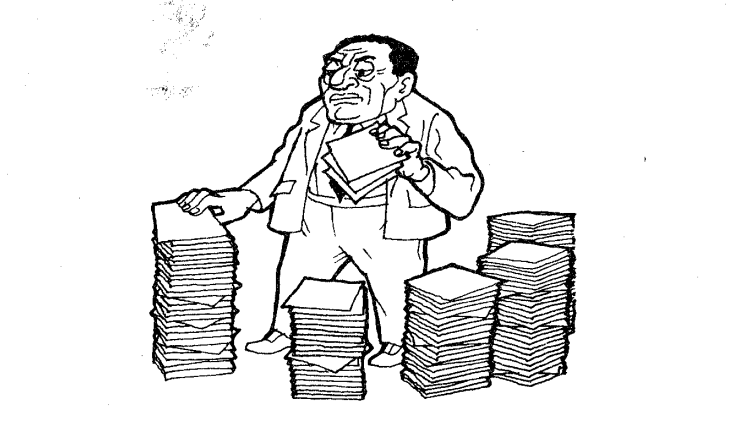
\includegraphics[scale=0.9]{./estáticos/ordenacionFicheros.png}
\caption{Ordenación de ficheros}
\end{figure}

\section{Ordenación por mezcla (Merge Sort)}
El algoritmo de ordenación por mezcla es un algoritmo recursivo que se basa en la técnica de dividir y conquistar. Este algoritmo consiste en dividir el arreglo a ordenar en varias partes, estas partes se ordenan y, posteriormente, se mezclan entre ellas de forma ordenada. Dado que el proceso de mezcla es menos costoso que el proceso de ordenación obtenemos un algoritmo más eficiente.

El algoritmo de ordenación por mezcla se basa en los siguientes principios:
\begin{enumerate}
    \item Dividir recursivamente el arreglo en 2 partes.
    \item Si el arreglo tiene un solo elemento, entonces está ordenado por definición.
    \item Si la lista tiene más de un ítem, dividimos la lista e invocamos recursivamente un ordenamiento por mezcla para ambas mitades.
    \item Una vez que ambas mitades estén ordenadas, la operación de mezcla se encarga de unir ambas mitades en un solo arreglo ordenado.
\end{enumerate}

El proceso de división puede verse de la siguiente manera:

\newpage
\begin{figure}[h]
\centering
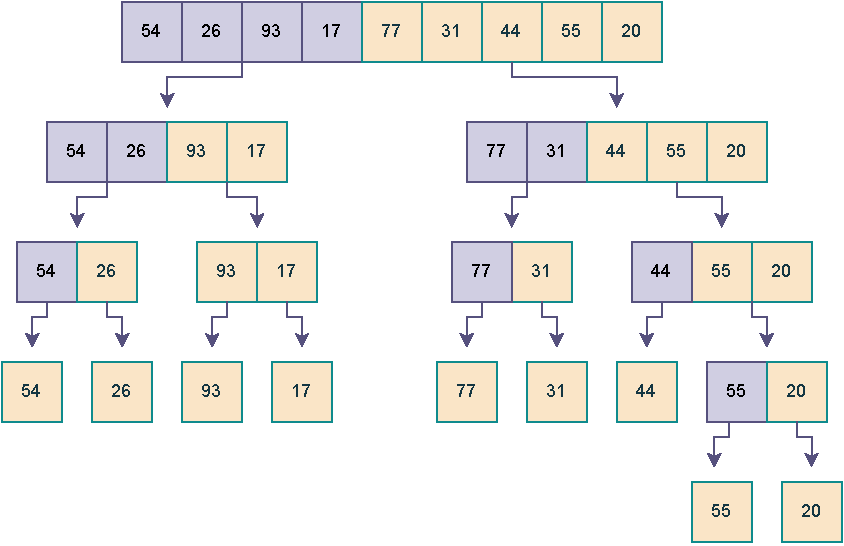
\includegraphics[scale=0.88]{./estáticos/mergediv.pdf}
\caption{Ejemplo de proceso de división}
\end{figure}

El proceso de mezcla puede verse de la siguiente manera:

\begin{figure}[h]
\centering
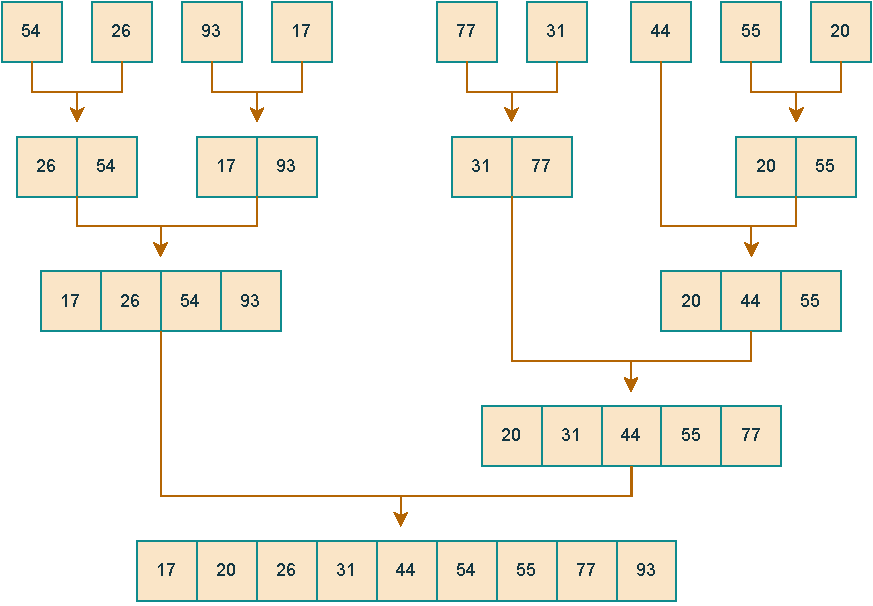
\includegraphics[scale=0.88]{./estáticos/mergemezcla.pdf}
\caption{Ejemplo de proceso de mezcla}
\end{figure}

\subsection{Idea de crear el código}
La idea es definir un procedimiento al que le pasamos en qué parte del arreglo queremos hacer lo fundamental del mergesort: dividirlo en dos, ordenar cada mitad y luego intercalar las dos mitades. Este procedimiento es \texttt{merge\_sort\_rec}, que toma el arreglo a y las posiciones inicial y final del pedazo de arreglo que vamos a ordenar. El procedimiento principal llama al recursivo con los índices 1 y n (el arreglo completo).

\begin{codebox}{Código 26}
\footnotesize Estructura de la función merge\_sort
\tcblower
\begin{pascallike}
proc merge_sort(in/out a: array[1..n] of T)
    merge_sort_rec(a,1,n)
end proc
proc merg_sort_rec(in/out a: array[1..n] of T, in lft,rgt: nat)
...
end proc
\end{pascallike}
\end{codebox}

El procedimiento \texttt{merge\_sort\_rec} toma el arreglo a, y los índices \textbf{lft} y \textbf{rgt}, que corresponden con el comienzo y el final del pedazo de arreglo que queremos ordenar. Recordando la idea del algoritmo, el caso más simple es cuando el pedazo de arreglo tiene un solo elemento. En nuestra implementación eso corresponde a que lft sea igual a rgt. En ese caso el procedimiento no debe hacer nada, ya que el pedazo está trivialmente ordenado.
En caso que no se dé esa situación, debemos:
\begin{enumerate}
    \item Dividir el pedazo de arreglo en dos,
    \item ordenar cada una de esas mitades utilizando el mismo algoritmo, e
    \item intercalar cada mitad ordenada.
\end{enumerate}
Para dividir el pedazo de arreglo, se define una variable \textbf{mid} de tipo nat a la que se le asigna el índice correspondiente a la posición del medio.

\begin{codebox}{Código 27}
\footnotesize División del arreglo
\tcblower
\begin{pascallike}
proc merg_sort_rec(in/out a: array[1..n] of T, in lft,rgt: nat)
    var mid: nat
    if rgt > lft --> mid := (rgt+lft) `div` 2
    ...
end proc
\end{pascallike}
\end{codebox}
Ahora entonces hay que llamar recursivamente al procedmiento dos veces: una para la primera mitad que irá desde la posición \textbf{lft} hasta \textbf{mid}, y otra para la segunda mitad, que irá desde la posición \textbf{mid+1} hasta \textbf{rgt}.
\begin{codebox}{Código 28}
\footnotesize Llamada recursiva
\tcblower
\begin{pascallike}
proc merg_sort_rec(in/out a: array[1..n] of T, in lft,rgt: nat)
    var mid: nat
    if rgt > lft --> mid := (rgt+lft) `div` 2
    merge_sort_rec(a,lft,mid)
    merge_sort_rec(a,mid+1,rgt)
    ...
end proc
\end{pascallike}
\end{codebox}
y por último, hay que intercalar. Esta tarea la implementaremos con un procedimiento llamado \texttt{merge}, que se define mas adelante.
\begin{codebox}{Código 29}
\footnotesize Definición completa de la función merge\_sort\_rec
\tcblower
\begin{pascallike}
proc merg_sort_rec(in/out a: array[1..n] of T, in lft,rgt: nat)
    var mid: nat
    if rgt > lft --> mid := (rgt+lft) `div` 2
    merge_sort_rec(a,lft,mid)
    merge_sort_rec(a,mid+1,rgt)
    merge(a,lft,mid,rgt)
end proc
\end{pascallike}
\end{codebox}
Ahora para implementar el procedimiento de \textbf{intercalación}, se necesita un arreglo auxiliar, en donde se van a guardar los valores de la primera mitad a intercalar.
Se define entonces una variable de tipo array, dos variables en las que luego almacenaremos índices \texttt{j} y \texttt{k}, y se copia la primera mitad del arreglo en el arreglo auxiliar:
\begin{codebox}{Código 30}
\footnotesize Inicialización de variables
\tcblower
\begin{pascallike}
proc merge(in/out a: array[1..n] of T, in lft,mid,rgt: nat)
    var tmp: array[1..n] of T
    var j,k: nat
    for i:=lft to mid do ->
        tmp[i] := a[i] 
    od
    ...
end proc
\end{pascallike}
\end{codebox}
Los índices \texttt{j} y \texttt{k} indicarán respectivamente el elemento de la primera mitad que estoy analizando para insertar en el pedazo de arreglo que quedará ordenado, y el índice de la segunda mitad que estoy analizando. Inicialmente observo el primero de cada mitad, es decir \textbf{lft} y \textbf{mid+1}.
\begin{codebox}{Código 31}
\footnotesize Inicialización de índices
\tcblower
\begin{pascallike}
proc merge(in/out a: array[1..n] of T, in lft,mid,rgt: nat)
    var tmp: array[1..n] of T
    var j,k: nat
    for i:=lft to mid do ->
        tmp[i] := a[i] 
    od
    j := lft
    k := mid+1
    ...
end proc
\end{pascallike}
\end{codebox}
Ahora hay que rellenar el pedazo completo de arreglo que contendrá las dos mitades intercaladas ordenadamente. Lo recorro con un for desde lft hasta rgt. Y se puede ver que en cada paso si el elemento que estoy observando de la primera mitad es menor o igual que el de la segunda mitad, de acuerdo a esa comparación sabré qué elemento va a ubicarse en el arreglo ordenado.
\begin{codebox}{Código 32}
\footnotesize Intercalación
\tcblower
\begin{pascallike}
proc merge(in/out a: array[1..n] of T, in lft,mid,rgt: nat)
    var tmp: array[1..n] of T
    var j,k: nat
    for i:=lft to mid do ->
        tmp[i] := a[i] 
    od
    j := lft
    k := mid+1
    for i:=lft to rgt do ->
        if j <= mid && (k > rgt || tmp[j] <= a[k])
            then a[i] := tmp[j]
                j:= j+1
            else a[i] := a[k]
                k := k+1
        fi
    od
end proc
\end{pascallike}
\end{codebox}
En la guarda del if hay que considerar también el caso en que ya haya agotado todos los elementos de la segunda mitad, lo que sucederá cuando \texttt{k > rgt}, y entonces en ese caso también completo con los elementos de la primera mitad (es decir los que están en el arreglo auxiliar).

\subsection{Análisis de complejidad}
Para analizar la función, debemos considerar los dos procesos distintos que conforman su implementación. En primer lugar, la lista se divide en mitades. Podemos dividir una lista por la mitad en un tiempo $\log n$ donde $n$ es la longitud de la lista. El segundo proceso es la mezcla. Cada ítem de la lista se procesará y se colocará en la lista ordenada. Así que la operación de mezcla que da lugar a una lista de tamaño n requiere n operaciones. El resultado de este análisis es que se hacen $\log n$ divisiones, cada una de las cuales cuesta $n$ para un total de $n\log n$ operaciones. Un ordenamiento por mezcla es un algoritmo $O(n \log n)$.

\subsection{Código}

\begin{codebox}{Código 33}
\footnotesize Ordenación por mezcla (Merge Sort)
\tcblower
\begin{pascallike}
proc merge_sort(in/out a: array[1..n] of T)
    merge_sort_rec(a,1,n)
end proc

proc merge_sort_rec(in/out a: array[1..n] of T, in lft,rgt: nat)
    var mid: nat
    if rgt > lft --> mid := (rgt+lft) `div` 2
        merge_sort_rec(a,lft,mid)
        merge_sort_rec(a,mid+1,rgt)
        merge(a,lft,mid,rgt)
    fi
end proc

proc merge(in/out a: array[1..n] of T, in lft,mid,rgt: nat)
    var tmp: array[1..n] of T
    var j,k: nat
    for i:=lft to mid do ->
        tmp[i] := a[i] 
    od
    j := lft
    k := mid+1
    for i:=lft to rgt do ->
        if j <= mid && (k > rgt || tmp[j] <= a[k])
            then a[i] := tmp[j]
                j:= j+1
            else a[i] := a[k]
                k := k+1
        fi
    od
end proc
\end{pascallike}
\end{codebox}

\section{Ordenación rápida (Quick Sort)}
El ordenamiento rápido usa dividir y conquistar para obtener las mismas ventajas que el ordenamiento por mezcla, pero sin utilizar almacenamiento adicional. Sin embargo, es posible que la lista no se divida por la mitad. Cuando esto sucede, el desempeño disminuye.

El algoritmo de ordenación rápida se basa en los siguientes principios:
\begin{enumerate}
    \item Primero selecciona un valor, que se denomina el \textbf{pivot} (El papel del valor pivote es ayudar a dividir la lista).
    \item La posición real a la que pertenece el valor pivote en la lista final ordenada, comúnmente denominado punto de división, se utilizará para dividir la lista para las llamadas posteriores a la función de ordenamiento rápido.
    \item El proceso de partición sucederá a continuación. Encontrará el punto de división y al mismo tiempo moverá otros ítems al lado apropiado de la lista, según sean menores o mayores que el valor pivote.
\end{enumerate}

A modo ilustrativo, se puede ver el proceso de partición en la siguiente figura:

\begin{figure}[h]
\centering
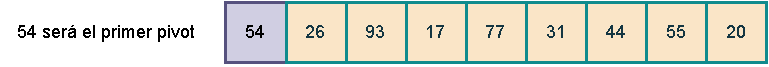
\includegraphics[scale=0.88]{./estáticos/pivot.pdf}
\caption{Ejemplo de proceso de partición}
\end{figure}

El particionamiento comienza localizando dos marcadores de posición \texttt{lft} y \texttt{rgt} al principio y al final de los ítems restantes de la lista. El objetivo del proceso de partición es mover ítems que están en el lado equivocado con respecto al valor pivote mientras que también se converge en el punto de división.

\begin{figure}[h]
\centering
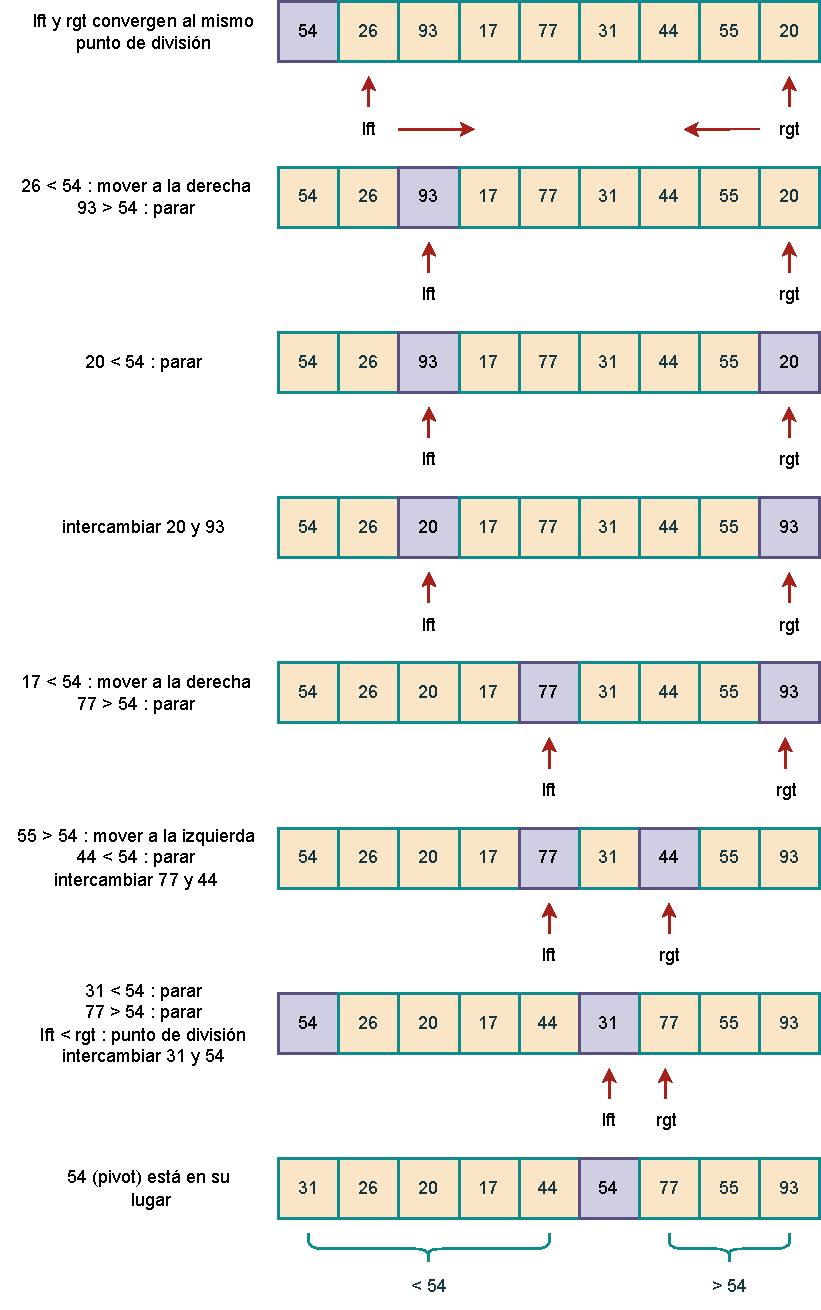
\includegraphics[scale=0.74]{./estáticos/quick.pdf}
\caption{Ejemplo de proceso}
\end{figure}

\begin{itemize}
    \item Comienza incrementando \texttt{lft} hasta que localicemos un valor que sea mayor que el valor pivote. Luego decrementamos \texttt{rgt} hasta que encontremos un valor que sea menor que el valor pivote. En tal punto habremos descubierto dos ítems que están fuera de lugar con respecto al eventual punto de división. 
    \item Para este ejemplo, esto ocurre en 93 y 20. Ahora se deben intercambiar estos dos ítems y luego repetir el proceso de nuevo.
    \item Se detiene en el punto donde \texttt{rgt} se vuelva menor que \texttt{lft}. La posición de \texttt{lft} es ahora el punto de división. El valor pivote se puede intercambiar con el contenido del punto de división y el valor pivote está ahora en su lugar.
\end{itemize}
\textit{ La lista ahora se puede dividir en el punto de división y el ordenamiento rápido se puede invocar recursivamente para las dos mitades.}

\subsection{Idea de crear el código}
De manera similar al algoritmo de ordenación \texttt{merge\_sort}, se define un procedimiento recursivo que tomará el arreglo de elementos y dos índices correspondientes al pedazo de arreglo que se ordenará. El algoritmo principal llama a este procedimiento con los índices \texttt{1} y \texttt{n}, correspondiendo con la ordenación del arreglo completo.

\begin{codebox}{Código 34}
\footnotesize Estructura de la función quick\_sort
\tcblower
\begin{pascallike}
proc quick_sort(in/out a: array[1..n] of T)
    quick_sort_rec(a,1,n)
end proc
proc quick_sort_rec(in/out a: array[1..n] of T, in lft,rgt: nat)
...
end proc
\end{pascallike}
\end{codebox}
Este procedimiento recursivo tiene su caso más simple cuando \textbf{lft} y \textbf{rgt} son iguales, lo que significa que estoy ordenando un arreglo de un solo elemento. En el caso interesante, al procedimiento se lo llama partition que será el encargado de acomodar los elementos del pedazo de arreglo utilizando el elemento de más a la izquierda como \textbf{pivot}.
\begin{codebox}{Código 35}
\footnotesize Llamada a la función partition
\tcblower
\begin{pascallike}
proc quick_sort_rec(in/out a: array[1..n] of T, in lft,rgt: nat)
    var ppiv: nat
    if rgt > lft --> 
        partition(a,lft,rgt,ppiv)
    ...
...
end proc
\end{pascallike}
\end{codebox}
El procedimiento \texttt{partition} modifica el arreglo desde \texttt{lft} hasta \texttt{rgt} dejando al comienzo todos los elementos que son menores o iguales al que se encontraba originalmente en la posición \texttt{lft}, y al final a todos los que son mayores o iguales. También modifica la variable \texttt{ppiv} asignándole el índice correspondiente al lugar donde queda ubicado definitivamente el elemento que se usó como \textbf{pivot}.
Luego lo único que queda por hacer es llamar recursivamente al procedimiento, una vez para los elementos que quedaron acomodados a la izquierda del pivot, y otra vez para los elementos que quedaron acomodados a la derecha.
\begin{codebox}{Código 36}
\footnotesize Llamada recursiva
\tcblower
\begin{pascallike}
proc quick_sort_rec(in/out a: array[1..n] of T, in lft,rgt: nat)
    var ppiv: nat
    if rgt > lft --> 
        partition(a,lft,rgt,ppiv)
        quick_sort_rec(a,lft,ppv-1)
        quick_sort_rec(a,ppiv+1,rgt)
    fi
end proc
\end{pascallike}
\end{codebox}
Queda por ver el procedimiento partition. Toma el arreglo, los dos índices que indican qué fragmento estamos ordenando, y una variable de solo escritura, en la cual indicaremos el índice en donde queda el pivot una vez que finalice el procedimiento.

\begin{codebox}{Código 37}
\footnotesize Estructura de la función partition
\tcblower
\begin{pascallike}
proc partition(in/out a: array[1..n] of T, in lft,rgt: nat, out ppiv: nat)
...
end proc
\end{pascallike}
\end{codebox}
Lo que hay que hacer en este procedimiento es ir mirando con un índice los elementos que están a la izquierda y con otro los que están a la derecha. El índice \texttt{i} indicará el elemento que estoy mirando desde la izquierda, y respectivamente \texttt{j} indicará el de la derecha. El elemento tomado como \textbf{pivot} será el que está más a la izquierda.
\begin{codebox}{Código 38}
\footnotesize Inicialización de variables
\tcblower
\begin{pascallike}
proc partition(in/out a: array[1..n] of T, in lft,rgt: nat, out ppiv: nat)
    var i,j: nat
    ppiv:= lft
    i:= lft+1
    j:= rgt
    ...
end proc
\end{pascallike}
\end{codebox}
Luego hay que ir viendo si el elemento indicado con el índice \texttt{i} y el indicado con \texttt{j} están bien ubicados, es decir, si \texttt{a[i]} es menor o igual al \textbf{pivot}, y si \texttt{a[j]} es mayor o igual. En caso que sea así, \texttt{"avanzo"} el índice. Este avance corresponde a sumar uno para \texttt{i}, y a restar uno para \texttt{j}. En caso que el elemento de la izquierda esté mal ubicado, debemos encontrar un elemento de la derecha que también esté mal ubicado, y los intercambiamos.
\begin{codebox}{Código 39}
\footnotesize Particionamiento
\tcblower
\begin{pascallike}
proc partition(in/out a: array[1..n] of T, in lft,rgt: nat, out ppiv: nat)
    var i,j: nat
    ppiv:= lft
    i:= lft+1
    j:= rgt
    do i <= j -->
        if a[i] <= a[ppiv] --> i:= i+1
            a[j] >= a[ppiv] --> j:= j-1
            a[i] > a[ppiv] && a[j] < a[ppiv] --> swap(a,i,j)
        fi
    od
...
end proc
\end{pascallike}
\end{codebox}
Esto se repite hasta que los índices \texttt{i} y \texttt{j} se hayan cruzado. En ese momento se termina el ciclo y solo queda ubicar correctamente al elemento \textbf{pivot}, y asignar la variable \texttt{ppiv} para que indique la posición final en donde queda el mismo.

\begin{codebox}{Código 40}
\footnotesize Finalización del procedimiento
\tcblower
\begin{pascallike}
proc partition(in/out a: array[1..n] of T, in lft,rgt: nat, out ppiv: nat)
    var i,j: nat
    ppiv:= lft
    i:= lft+1
    j:= rgt
    do i <= j --> if a[i] <= a[ppiv] --> i:= i+1
                        a[j] >= a[ppiv] --> j:= j-1
                        a[i] > a[ppiv] && a[j] < a[ppiv] --> swap(a,i,j)
                    fi
    od
    swap(a,ppiv,j)
    ppiv:= j
end proc
\end{pascallike}
\end{codebox}

\subsection{Análisis de complejidad}
Para analizar la función, hay que tener en cuenta que para una lista de longitud $n$, si la partición siempre ocurre en el centro de la lista, habrá de nuevo $\log n$ divisiones. Con el fin de encontrar el punto de división, cada uno de los $n$ ítems debe ser comparado contra el valor pivote. El resultado es $n\log n$ . Además, no hay necesidad de memoria adicional como en el proceso de ordenamiento por mezcla.
En el peor de los casos, los puntos de división pueden no estar en el centro y podrían estar muy sesgados a la izquierda o a la derecha, dejando una división muy desigual. En este caso, ordenar una lista de $n$ ítems se divide en ordenar una lista de $0$ ítems y una lista de $n-1$ ítems. Similarmente, ordenar una lista de tamaño $n-1$ se divide en una lista de tamaño $0$ y una lista de tamaño $n-2$ y así sucesivamente. El resultado es un ordenamiento $O(n^2)$ con toda la sobrecarga que requiere la recursión.

\subsection{Código}

\begin{codebox}{Código 41}
\footnotesize Ordenación rápida (Quick Sort)
\tcblower
\begin{pascallike}
proc quick_sort(in/out a: array[1..n] of T)
    quick_sort_rec(a,1,n)
end proc

proc quick_sort_rec(in/out a: array[1..n] of T, in lft,rgt: nat)
    var ppiv: nat
    if rgt > lft --> 
        partition(a,lft,rgt,ppiv)
        quick_sort_rec(a,lft,ppv-1)
        quick_sort_rec(a,ppiv+1,rgt)
    fi
end proc

proc partition(in/out a: array[1..n] of T, in lft,rgt: nat, out ppiv: nat)
    var i,j: nat
    ppiv:= lft
    i:= lft+1
    j:= rgt
    do i <= j --> if a[i] <= a[ppiv] --> i:= i+1
                        a[j] >= a[ppiv] --> j:= j-1
                        a[i] > a[ppiv] && a[j] < a[ppiv] --> swap(a,i,j)
                    fi
    od
    swap(a,ppiv,j)
    ppiv:= j
end proc
\end{pascallike}
\end{codebox}
\chapter{Recurrencias Divide y Vencerás}
Un algoritmo Divide y Vencerás típico resuelve un problema siguiendo estos 3 pasos:
\begin{enumerate}
    \item \textbf{Dividir:} Descomponer el problema en sub-problemas del mismo tipo. Este paso involucra descomponer el problema original en pequeños sub-problemas. Cada sub-problema debe representar una parte del problema original. Por lo general, este paso emplea un enfoque recursivo para dividir el problema hasta que no es posible crear un sub-problema más.
    \item \textbf{Vencer:} Resolver los sub-problemas recursivamente. Este paso recibe un gran conjunto de sub-problemas a ser resueltos. Generalmente a este nivel, los problemas se resuelven por sí solos.
    \item \textbf{Combinar:}  Combinar las respuestas apropiadamente. Cuando los sub-problemas son resueltos, esta fase los combina recursivamente hasta que estos formulan la solución al problema original. Este enfoque algorítmico trabaja recursivamente y los pasos de conquista y fusión trabajan tan a la par que parece un sólo paso.
\end{enumerate}

\section{Estructura de un algoritmo Divide y Vencerás}
La estrucutra de un algoritmo utilizado esta técnica es la siguiente:

\begin{codebox}{Código 42}
\footnotesize Divide y Vencerás
\tcblower
\begin{verbatim}
fun DyV(x) ret y
    if x suficientemente pequeño o simple then y:= ad_hoc(x)
    else descomponer x en x1, x2, . . . , xa
        for i:= 1 to a do 
            yi := DyV(xi) 
        od
        combinar y1, y2, . . . , ya para obtener la solución y de x
    fi
end fun
\end{verbatim}
\end{codebox}
Donde normalmente $x_i$ es una fracción de $x$ ($|x_i| = \frac{|x|}{b}$), para algun $b$ constante mayor a 1).

Normalmente se ve lo siguiente:
\begin{itemize}
    \item \textbf{Solución trivial}: Si el problema es suficientemente pequeño, se resuelve de manera directa.
    \item \textbf{Descomposisión}: Se divide el problema en subproblemas más pequeños.
    \item \textbf{Combinación}: Se combinan las soluciones de los subproblemas para obtener la solución del problema original.
\end{itemize}

\section{Ejemplos}
\begin{enumerate}
    \item Ordenación por intercalación
    \begin{itemize}
        \item \textbf{Solución trivial}: Si el arreglo tiene un solo elemento, ya está ordenado.
        \item \textbf{Descomposición}: Se divide el arreglo en dos mitades ($b=2$).
        \item \textbf{Combinación}: Se intnercalan los dos arreglos ordenados.
    \end{itemize}
    \item Ordenación rápida
    \begin{itemize}
        \item \textbf{Solución trivial}: Si el arreglo tiene un solo elemento, ya está ordenado.
        \item \textbf{Descomposición}: Se elige un pivote y se divide el arreglo en dos partes, una con los elementos menores al pivote y otra con los elementos mayores ($b=2$).
        \item \textbf{Combinación}: Se ordenan las dos partes recursivamente.
    \end{itemize}
\end{enumerate}

\section{Análisis de algoritmos Divide y Vencerás}
Si queremos contar el costo computacional (número de operaciones) $t(n)$ de la función $DyV$ obtenemos:
\begin{equation*}
    t(n) = 
    \begin{cases}
        c & \text{si la entrada es pequeña o simple} \\
        a \cdot t(n/b) + g(n) & \text{en caso contrario}
    \end{cases}
\end{equation*}
Donde:
\begin{itemize}
    \item $c$ es una constante que representa el costo computacional de la función \texttt{ad\_hoc} en el caso base.
    \item $a \cdot t(n/b)$, el valor $a$ que representa la cantidad de llamadas recursivas por nivel y $n/b$ es el tamaño de la entrada en cada llamada recursiva es decir, el tamaño de los subproblemas.
    \item $g(n)$ es el costo computacional de los procesos de descomposición y de combinación.
\end{itemize}

Si $t(n)$ no es decreciente, y $g(n)$ es polinomial, entonces:
\begin{equation*}
    t(n) = 
    \begin{cases}
        n ^{\log_ba} & \text{si } a > b^k \\
        n^k \log n & \text{si } a = b^k \\
        n^k & \text{si } a < b^k
    \end{cases}
\end{equation*}

\section{Ejemplo completo de análisis}
Se busca calcular el orden de complejidad de:
\begin{codebox}{Código 43}
\footnotesize Ejemplo completo
\tcblower
\begin{pascallike}
proc f1(in n : nat)
    if n $\leq$ 1 then skip
    else
        for i := 1 to 8 do f1(n div 2) od
        for i := 1 to n 3 do t := 1 od
    fi
end proc
\end{pascallike}
\end{codebox}
En este caso notar que:
\begin{itemize}
    \item Tamaño de la entrada: $n$,
    \item Operación a contar: $t := 1$.
\end{itemize}
Entonces, se puede definir una funcion $r(n)$, que representará la cantidad de asignaciones a la variable $t$ que ocurren al llamar a la función $f1$ con el dato de entrada $n$.

Podemos observar que la función $f1$ esta dividida en dos casos, si $n \leq 1$ entonces no se realiza ninguna asignación a la variable $t$, por lo que $r(n) = 0$.
\begin{equation*}
    r(n) = 
    \begin{cases}
        0 & \text{si } n \leq 1 \\
        ... & \text{en caso contrario}
    \end{cases}
\end{equation*}
Como hay dos ciclos for en una secuencia, se puede analizar cada uno por separado y sumarlos, por ahora los puedo expresar como sumatoria:
\begin{equation*}
    r(n) = 
    \begin{cases}
        0 & \text{si } n \leq 1 \\
        \sum_{i=1}^{8} ... + \sum_{i=1}^{n^3} ... & \text{en caso contrario}
    \end{cases}
\end{equation*}
En el primer for, queremos contar la cantidad de asignaciones que se realizan al llamar a la función $f1$ con el dato de entrada $n/2$, por lo que se puede expresar como:
\begin{equation*}
    r(n) = 
    \begin{cases}
        0 & \text{si } n \leq 1 \\
        \sum_{i=1}^{8} r(n/2) + \sum_{i=1}^{n^3} ... & \text{en caso contrario}
    \end{cases}
\end{equation*}
En el segundo for, se realiza una asignación a la variable $t$ por cada iteración, por lo que se puede expresar como:
\begin{equation*}
    r(n) = 
    \begin{cases}
        0 & \text{si } n \leq 1 \\
        \sum_{i=1}^{8} r(n/2) + \sum_{i=1}^{n^3} 1 & \text{en caso contrario}
    \end{cases}
\end{equation*}
Resolviendo las sumatorias, se obtiene:
\begin{equation*}
    r(n) = 
    \begin{cases}
        0 & \text{si } n \leq 1 \\
        8 \cdot r(n/2) + n^3 & \text{en caso contrario}
    \end{cases}
\end{equation*}
Por lo que se puede observar que:
\begin{itemize}
    \item $a = 8$,
    \item $b = 2$,
    \item $g(n) = n^3$.
\end{itemize}
Como $a = 8 = 2^3 = b^3$, se puede decir que el orden de complejidad es $O(n^3 \log n)$.
\chapter{Tipos concretos}
Se van a presentar los tipos enumerados, tuplas, arreglos y punteros.

\section{Tipos enumerados}
Los tipos enumerados son aquellos que permiten definir un conjunto finito de valores, los cuales son llamados elementos del tipo. En Pascal, se definen de la siguiente manera:
\begin{codebox}{Código 44}
\footnotesize Definición de un tipo enumerado
\tcblower
\begin{pascallike}
type E = enumerate
            elem1
            elem2
            ...
            elemk;
        end enumerate;
\end{pascallike}
\end{codebox}
En esta definición el tipo E tiene $k$ elementos, los cuales son $elem1, elem2, ..., elemk$, si se quiere utilizar este tipo, en un programa se puede declarar una variable de tipo E y asignarle uno de los elementos del tipo.
\begin{codebox}{Código 45}
\footnotesize Declaración de una variable de tipo enumerado
\tcblower
\begin{pascallike}
var v : E;
v := elem1;
\end{pascallike}
\end{codebox}
Por defecto en el lenguaje de la materia, vamos a poder utilizar los tipos enumerados con orden, es decir, podemos con un ciclo for recorrer todos los elementos del tipo enumerado:
\begin{codebox}{Código 46}
\footnotesize Recorrido de un tipo enumerado
\tcblower
\begin{pascallike}
for v := elem1 to elemk do ... od
\end{pascallike}
\end{codebox}

\section{Tuplas}
Las tuplas son un tipo de dato que permite agrupar varios valores en una sola variable. En el lenguaje de la materia, las tuplas se definen de la siguiente manera:
\begin{codebox}{Código 47}
\footnotesize Definición de una tupla
\tcblower
\begin{pascallike}
type Tupla = tuple
                campo1 : tipo1;
                campo2 : tipo2;
                ...
                campok : tipok;
            end tuple;
\end{pascallike}
\end{codebox}
En esta definición, la tupla Tupla tiene $k$ campos, los cuales son campo1, campo2, ..., campok, cada campo tiene un tipo asociado, el cual puede ser cualquier tipo de dato. Para acceder a los campos de una tupla se utiliza el operador punto.

Por ejemplo, se quiere definir un tipo para persona y luego acceder a los campos de la persona:
\begin{codebox}{Código 48}
\footnotesize Definición de una tupla y acceso a los campos
\tcblower
\begin{pascallike}
type Persona = tuple
                name: string
                age: nat
                weight: real
            end tuple;
var p: Persona;
p.name := "Juan";
p.age := 20;
p.weight := 70.5;
\end{pascallike}
\end{codebox}

\section{Arreglos}
Los arreglos son un tipo de dato que permite almacenar varios valores del mismo tipo en una sola variable de tamaño fijo. En el lenguaje de la materia, los arreglos se definen de la siguiente manera:
\begin{codebox}{Código 49}
\footnotesize Definición de un arreglo
\tcblower
\begin{pascallike}
var arr = array[M..N] of T;
\end{pascallike}
\end{codebox}
En esta definición, arr es un arreglo de tamaño $N-M$ de elementos de tipo T, los índices del arreglo van desde M hasta N. Para acceder a los elementos de un arreglo se utiliza el operador corchetes.

Tambien se puede definir un arreglo cuyos índices sean de tipo enumerado:
\begin{codebox}{Código 50}
\footnotesize Definición de un arreglo con índices de tipo enumerado
\tcblower
\begin{pascallike}
type E = enumerate
            elem1
            elem2
            ...
            elemk;
        end enumerate;
var arr = array[elem1..elemk] of T;
\end{pascallike}
\end{codebox}
Si se busca crear arreglos de mas de una dimension, simplemente se separan por comas los tamaños de las dimensiones:
\begin{codebox}{Código 51}
\footnotesize Definición de un arreglo de dos dimensiones
\tcblower
\begin{pascallike}
var arr = array[M1..N1, M2..N2] of T;
\end{pascallike}
\end{codebox}
Y el acceso a los elementos de un arreglo de dos dimensiones se hace de la siguiente manera:
\begin{codebox}{Código 52}
\footnotesize Acceso a los elementos de un arreglo de dos dimensiones
\tcblower
\begin{pascallike}
arr[i, j] := 5;
\end{pascallike}
\end{codebox}
donde i es el índice de la primera dimensión y j es el índice de la segunda dimensión.

\section{Punteros}
Dado un tipo T, un puntero a T es un tipo de datos que representa el lugar en la memoria en donde está alojado un elemento de tipo T. Por ejemplo, se puede definir un puntero a un natural de la siguiente manera:
\begin{codebox}{Código 53}
\footnotesize Definición de un puntero
\tcblower
\begin{pascallike}
var p: pointer to nat;
\end{pascallike}
\end{codebox}

\subsection{Operaciones con punteros}
\begin{enumerate}
    \item \textbf{Reservar:} Para reservar un nuevo bloque de memoria donde pueda almacenar un elemento del tipo al que apunta se utiliza la operación \texttt{alloc}.
    \item \textbf{Acceder al valor:} Puedo acceder al valor en el bloque de memoria apuntado por p mediante la operación $\star$. Por ejemplo \texttt{$\star p := 10$} decimos que el valor al que apunta p es 10.
    \item \textbf{Liberar:} Para liberar el bloque de memoria reservado se utiliza la operación \texttt{free}. Por ejemplo \texttt{free(p)}, decimos que $p$ ya no apunta a ningún bloque de memoria.
\end{enumerate}
Para representar punteros que no apunten a nada se utiliza el valor \texttt{null}. Por ejemplo, si se quiere inicializar un puntero a nat que no apunte a nada se puede hacer de la siguiente manera:
\begin{codebox}{Código 54}
\footnotesize Inicialización de un puntero a nat
\tcblower
\begin{pascallike}
var p: pointer to nat;
p := null;
\end{pascallike}
\end{codebox}

\subsection{Ejemplo de uso de punteros}
Se tiene el tipo persona y se quiere crear un puntero a persona:
\begin{codebox}{Código 55}
\footnotesize Definición de un puntero a persona
\tcblower
\begin{pascallike}
type Persona = tuple
                name: string
                age: nat
                weight: real
            end tuple;
var p: pointer to Persona;
\end{pascallike}
\end{codebox}
Ahora se analizan los casos posibles para $p$:
\begin{figure}[h]
    \centering
    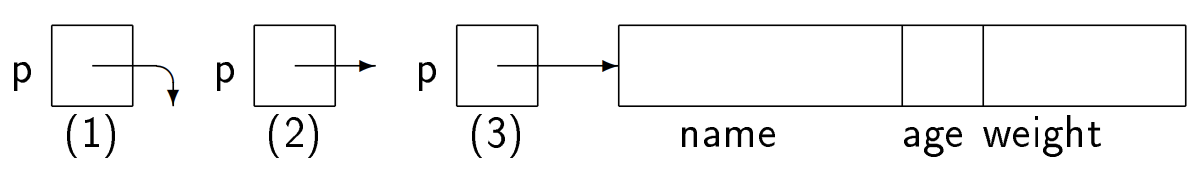
\includegraphics[scale=0.5]{./estáticos/punterosej.png}
    \caption{Casos posibles para un puntero}
    \label{fig:my_label}
\end{figure}
\begin{enumerate}
    \item El valor de $p$ es \texttt{null}, lo cual indica que no apunta a ningún bloque de memoria.
    \item La dirección de memoria a la que apunta $p$ no está reservada, por lo que no se puede acceder a ella.
    \item El valor de $p$ es una dirección de memoria reservada, por lo que se puede acceder a ella. En este caso, $\star p$ denota a la persona a la que apunta $p$ y por lo tanto se podria acceder a los campos de la persona ($\star$p.age, $\star$p.name, $\star$p.weight). Y tambien se podrian modificar los campos de la persona ($\star$p.age := 20).
\end{enumerate}
Una notación alternativa para acceder a los campos de una persona a la que apunta $p$ es $\rightarrow$, así por ejemplo en vez de $\star$p.age se puede escribir $p\rightarrow age$, tanto para leerlo como para modificarlo ($p\rightarrow age := 20$).


\chapter{Tipos Abstractos de Datos (TADs o ADTs en inglés)}

Un tipo abstracto de datos (TAD) es una colección de valores y operaciones que se definen mediante una especificación que es independiente de cualquier representación.

Un TAD es una abstracción:
\begin{itemize}
    \item Se destacan los detalles de la especificación (el qué),
    \item Se ocultan los detalles de la implementación (el cómo).
\end{itemize}

\section{Especificación de un TAD}
Para especificar un TAD se deben definir:
\begin{enumerate}
    \item Su \textbf{nombre}.
    \item Especificar \textbf{constructores}: procedimientos o funciones mediante los cuales puedo crear elementos del tipo que estoy especificando.
    \item Especificar \textbf{operaciones}: todos los procedimientos o funciones que permitirán manipular los elementos del tipo de datos que estoy especificando.
    \item Indicamos los \textbf{tipos} de cada constructor y operación (el encabezado de los procedimientos o funciones), y mediante lenguaje natural explicamos qué hacen.
    \item Algunas operaciones pueden tener restricciones que las indicamos mediante \textbf{precondiciones}.
    \item Debemos especificar también una operación de destrucción que libera la memoria utilizada por los elementos del tipo, en caso que sea necesario.
\end{enumerate}

\subsection{Ejemplo}
Suponga que se va a desarrollar un programa para administrar la información de una biblioteca.

Puesto que allí hay elementos como ficheros, usuarios, libros, etc., que participan en el problema, en el software existirá un TAD que represente y simule la operación de cada uno de ellos: el TAD Fichero, el TAD Usuario y el TAD Libro. Estos TAD estarán relacionados dentro del programa, de la misma manera como los elementos que modelan están relacionados en la biblioteca: un elemento del TAD Usuario puede tener en préstamo un elemento del TAD Libro, los elementos del TAD Fichero tienen elementos del TAD Ficha, que representan libros de la biblioteca, etc. No existirá un TAD Pared, puesto que no participa en el problema, así haga parte de la biblioteca (a menos, claro está, que se trate de un sistema de diseño arquitectónico, en el cual las paredes sean los elementos de base.

\section{Implementación de un TAD}
\begin{itemize}
    \item Definir un nuevo tipo con el nombre del TAD especificado. Para ello utilizamos tipos concretos y otros tipos definidos previamente.
    \item Implementar cada constructor respetando los tipos tal como fueron especificados.
    \item Implementar cada operación respetando los tipos tal como fueron especificados.
    \item Implementar operación de destrucción liberando memoria si es que se ha reservado al construir los elementos.
    \item Pueden surgir nuevas restricciones que dependen de cómo implementamos el tipo.
    \item Puedo necesitar operaciones auxiliares que no están especificadas en el tipo.
\end{itemize}

\section{TAD Lista}
Las listas son colecciones 0 o mas elementos de un mismo tipo, de tamaño variable.

\subsection{Especificación}
\begin{itemize}
    \item \textbf{Nombre}: Lista
    \item \textbf{Constructores}:
    \begin{itemize}
        \item \texttt{empty()}: crea una lista vacía. 
\begin{codebox}{Constructores}
\footnotesize empty()
\tcblower
\begin{pascallike}
fun empty() ret l : List of T
{- crea una lista vacia. -}
\end{pascallike}
\end{codebox}
        \item \texttt{addl()}: agrega un elemento al comienzo de la lista.
\begin{codebox}{Constructores}
\footnotesize addl()
\tcblower
\begin{pascallike}
proc addl (in e : T, in/out l : List of T)
{- agrega el elemento e al comienzo de la lista l. -}
\end{pascallike}
\end{codebox}
    \end{itemize}
    \item \textbf{Operaciones}:
    \begin{itemize}
        \item decidir si una lista es vacía,
        \item tomar el primer elemento,
        \item tirar el primer elemento,
        \item agregar un elemento al final,
        \item obtener la cantidad de elementos,
        \item concatenar dos listas,
        \item obtener el elemento en una posición específica,
        \item tomar una cantidad arbitraria de elementos,
        \item tirar una cantidad arbitraria de elementos,
        \item copiar una lista en una nueva.
    \end{itemize}
\end{itemize}

\begin{codebox}{TAD Lista}
\begin{pascallike}
spec List of T where

constructors    
    fun empty() ret l : List of T
    {- crea una lista vacia. -}

    proc addl (in e : T, in/out l : List of T)
    {- agrega el elemento e al comienzo de la lista l. -}

destroy
    proc destroy (in/out l : List of T)
    {- Libera memoria en caso que sea necesario. -}

operations
    fun is_empty(l : List of T) ret b : bool
    {- Devuelve True si l es vacia. -}

    fun head(l : List of T) ret e : T
    {- Devuelve el primer elemento de la lista l -}

    {- PRE: not is_empty(l) -}
    proc tail(in/out l : List of T)
    {- Elimina el primer elemento de la lista l -}

    {- PRE: not is_empty(l) -}
    proc addr (in/out l : List of T,in e : T)
    {- agrega el elemento e al final de la lista l. -}

    fun length(l : List of T) ret n : nat
    {- Devuelve la cantidad de elementos de la lista l -}

    proc concat(in/out l : List of T,in l0 : List of T)
    {- Agrega al final de l todos los elementos de l0
    en el mismo orden.-}

    fun index(l : List of T,n : nat) ret e : T
    {- Devuelve el n-esimo elemento de la lista l -}

    {- PRE: length(l) > n -}
    proc take(in/out l : List of T,in n : nat)
    {- Deja en l so lo los primeros n
    elementos, eliminando el resto -}

    proc drop(in/out l : List of T,in n : nat)
    {- Elimina los primeros n elementos de l -}

    fun copy_list(l1 : List of T) ret l2 : List of T
    {- Copia todos los elementos de l1 en la nueva lista l2 -}
\end{pascallike}
\end{codebox}

\subsection{Ejempo de uso}

\begin{codebox}{Promedio}
\footnotesize Uso de operaciones de listas
\tcblower
\begin{pascallike}
fun promedio (l : List of float) ret r : float
    var largo : nat
    var elem : float
    var laux : List of float

    laux := copy(l) {- copio la lista para no modificar la original -}
    r := 0.0 {- inicializo el promedio en 0 -}
    largo := length(laux) {- obtengo la cantidad de elementos -}
    do (not is_empty(laux)) -> {- mientras la lista no sea vacia -}
        elem := head(laux) {- tomo el primer elemento -}
        r := r + elem {- sumo el elemento al promedio -}
        tail(laux) {- elimino el primer elemento -}
    od
    destroy(laux) {- libero la memoria -}
    r := r / largo {- calculo el promedio -}
end proc
\end{pascallike}
\end{codebox}

\section{Implementación de un TAD Lista mediante punteros}
\begin{itemize}
    \item Implementaremos el TAD lista utilizando punteros, implementación conocida como \texttt{lista enlazada}.
    \item Cada elemento de la lista estará alojado en un nodo conteniendo además un puntero hacia el siguiente.
    \begin{figure}[h]
        \centering
        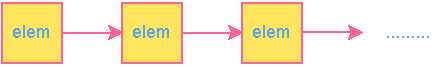
\includegraphics[scale=1]{./estáticos/node.pdf}
        \caption{Lista enlazada}
        \label{fig:my_label}
    \end{figure}
    \item Una lista será un puntero a un nodo.
    \item La lista vacía se implementa con el puntero null.
    \item Esta implementación permite tener la lista de elementos almacenada en lugares de la memoria no necesariamente contiguos.
    \item No existe límite teórico para almacenar elementos. En la práctica dicho límite será la cantidad de memoria.    
\end{itemize}

En resumen, la implementación de un TAD lista mediante punteros consiste en:
\begin{itemize}
    \item Definir un tipo nodo que contenga un elemento y un puntero al siguiente nodo.
    \item Definir un tipo lista que sea un puntero a un nodo.
    \item Implementar cada constructor y operación respetando los tipos especificados.
    \item Implementar la operación de destrucción liberando la memoria utilizada.
\end{itemize}

\textit{La implementación completa del TAD lista mediante punteros se encuentra en el solucionario.}

\section{TAD Contador}
Un problema interesante (y no del todo trivial) es el de controlar que una cierta expresión tiene balanceados sus paréntesis. Se quiere dar un algoritmo que tome una expresión (dada, por ejemplo, por un arreglo de caracteres) y devuelva verdadero si la expresión tiene sus paréntesis correctamente balanceados, y falso en caso contrario.
Este problema puede solucionarse con un algoritmo que recorre la expresión de izquierda a derecha y que utiliza un entero, que se inicializa en 0 y se incrementa cada vez que se encuentra un paréntesis que abre y se decrementa (chequeando previamente que dicho número no sea nulo) cada vez que se encuentra un paréntesis que cierra. Al analizar, sólo resta comprobar que dicho entero sea cero. Esta descripción debería alcanzar para darse uno cuenta de que no es en realidad un entero lo que hace falta, sino mucho menos. Un entero es un objeto que admite todas las operaciones aritméticas, acá sólo se necesita inicializar en 0, incrementar, decrementar y controlar si su valor es o no cero.

\subsection{Especificación}
Los \textbf{constructores} (en este caso inicial e incrementar) deben ser capaces de generar todos los valores posibles del TAD. En lo posible cada valor debe poder generarse de manera única. Intuitivamente, esto se cumple para inicial e incrementar: partiendo del valor inicial y tras sucesivos incrementos se puede alcanzar cualquier valor posible; y hay una única forma de alcanzar cada valor posible de esa manera.

Las demás \textbf{operaciones} quedan declaradas simplemente como tales. Las operaciones se definen con ecuaciones que deben cubrir todos los casos posibles, salvo los declarados que no pueden ocurrir, como en el caso de decrementar que no puede aplicarse a un contador que sea inicial (a pesar de que se podría defnir de manera obvia para ese caso). 
\begin{itemize}
    \item comprobar si su valor es el inicial
    \item decrementar si no lo es
\end{itemize}

\begin{codebox}{TAD Contador}
\begin{pascallike}
spec Counter where

constructors
    fun init() ret c : Counter
    {- crea un contador con valor inicial -}

    proc incr(in/out c : Counter)
    {- incrementa el valor del contador c -}

destroy
    proc destroy(in/out c : Counter)
    {- Libera memoria en caso que sea necesario. -}

operations
    fun is_init(c : Counter) ret b : bool
    {- Devuelve True si el contador c tiene el valor inicial -}

    {- PRE: not is_init(c) -}
    proc decr(in/out c : Counter)
    {- decrementa el valor del contador c -}
\end{pascallike}
\end{codebox}

\subsection{Implementación}

\begin{codebox}{Implementación del TAD Contador}
\begin{pascallike}
implement Counter where
type Counter = nat

proc init (out c: Counter)
    c:= 0
end proc

proc inc (in/out c: Counter)
    c:= c+1
end proc

fun is_init (c: Counter) ret b: bool
    b:= (c = 0)
end fun

{- PRE: not is_init(c) -}
proc dec (in/out c: Counter)
    c:= c-1
end proc

proc destroy (in/out c: Counter)
    skip
end proc
\end{pascallike}
\end{codebox}

\subsection{Algoritmo de balanceo de paréntesis}

\begin{codebox}{Algoritmo de balanceo de paréntesis}
\begin{pascallike}
fun matching_parenthesis (a: array[1..n] of char) ret b: bool
    var i: nat
    var c: Counter
    b:= true
    init(c)
    i:= 1
    do i $\leq$ n $\wedge$ b $\rightarrow$ if a[i] = '(' $\rightarrow$ inc(c)
                                    a[i] = ')' $\wedge$ is_init(c) $\rightarrow$ b:= false
                                    a[i] = ')' $\wedge$ $\neg$is_init(c) $\rightarrow$ dec(c)
                                    otherwise $\rightarrow$ skip
                                fi
                                i:= i+1
    od
    b:= b $\wedge$ is_init(c)
    destroy(c)
end fun
\end{pascallike}
\end{codebox}

\section{TAD Cola}

\subsection{Especificación}
\begin{itemize}
    \item \textbf{Nombre}: Cola
    \item \textbf{Constructores}:
    \begin{itemize}
        \item \texttt{empty()}: crea una cola vacía.
        \item \texttt{enqueue()}: agrega un elemento al final de la cola.
    \end{itemize}
    \item \textbf{Operaciones}:
    \begin{itemize}
        \item decidir si una cola es vacía,
        \item tomar el primer elemento,
        \item tirar el primer elemento,
        \item agregar un elemento al final,
        \item obtener la cantidad de elementos,
        \item copiar una cola en una nueva.
    \end{itemize}
\end{itemize}

\begin{codebox}{TAD Cola}
\begin{pascallike}
spec Queue of T where

constructors
    fun empty() ret q : Queue of T
    {- crea una cola vacia. -}

    proc enqueue(in e : T, in/out q : Queue of T)
    {- agrega el elemento e al final de la cola q. -}

destroy
    proc destroy(in/out q : Queue of T)
    {- Libera memoria en caso que sea necesario. -}

operations
    fun is_empty(q : Queue of T) ret b : bool
    {- Devuelve True si q es vacia. -}

    fun first(q : Queue of T) ret e : T
    {- Devuelve el primer elemento de la cola q -}

    {- PRE: not is_empty(q) -}
    proc dequeue(in/out q : Queue of T)
    {- Elimina el primer elemento de la cola q -}

    proc enqueue(in e : T, in/out q : Queue of T)
    {- agrega el elemento e al final de la cola q. -}

    fun length(q : Queue of T) ret n : nat
    {- Devuelve la cantidad de elementos de la cola q -}

    fun copy_queue(q1 : Queue of T) ret q2 : Queue of T
    {- Copia todos los elementos de q1 en la nueva cola q2 -}
\end{pascallike}
\end{codebox}

\subsection{Implementación}

\begin{codebox}{Implementación del TAD Cola}
\begin{pascallike}
implement Queue of T where
type Queue of T = record
    data: array[1..MAX] of T
    front: nat
    rear: nat
    size: nat
end record

proc empty (out q: Queue of T)
    q.front:= 1
    q.rear:= 0
    q.size:= 0
end proc

{- PRE: q.size < MAX -}
proc enqueue (in e: T, in/out q: Queue of T)
    q.rear:= (q.rear + 1) mod MAX
    q.data[q.rear]:= e
    q.size:= q.size + 1
end proc

fun is_empty (q: Queue of T) ret b: bool
    b:= (q.size = 0)
end fun

{- PRE: not is_empty(q) -}
proc dequeue (in/out q: Queue of T)
    q.front:= (q.front + 1) mod MAX
    q.size:= q.size - 1
end proc

fun first (q: Queue of T) ret e: T
    e:= q.data[q.front]
end fun

fun length (q: Queue of T) ret n: nat
    n:= q.size
end fun

fun copy_queue (q1: Queue of T) ret q2: Queue of T
    var i: nat
    q2.front:= 1
    q2.rear:= q1.size
    q2.size:= q1.size
    for i:= 1 to q1.size do
        q2.data[i]:= q1.data[(q1.front + i - 1) mod MAX]
    od
end fun

proc destroy (in/out q: Queue of T)
    skip
end proc
\end{pascallike}
\end{codebox}

\section{TAD Pila}

\subsection{Especificación}
\begin{itemize}
    \item \textbf{Nombre}: Pila
    \item \textbf{Constructores}:
    \begin{itemize}
        \item \texttt{empty()}: crea una pila vacía.
        \item \texttt{push()}: agrega un elemento al tope de la pila.
    \end{itemize}
    \item \textbf{Operaciones}:
    \begin{itemize}
        \item decidir si una pila es vacía,
        \item tomar el tope,
        \item tirar el tope,
        \item copiar una pila en una nueva.
    \end{itemize}
\end{itemize}

\begin{codebox}{TAD Pila}
\begin{pascallike}
spec Stack of T where

constructors
    fun empty() ret s : Stack of T
    {- crea una pila vacia. -}

    proc push(in e : T, in/out s : Stack of T)
    {- agrega el elemento e al tope de la pila s. -}

destroy
    proc destroy(in/out s : Stack of T)
    {- Libera memoria en caso que sea necesario. -}

operations
    fun is_empty(s : Stack of T) ret b : bool
    {- Devuelve True si s es vacia. -}

    fun top(s : Stack of T) ret e : T
    {- Devuelve el elemento del tope de la pila s -}

    {- PRE: not is_empty(s) -}
    proc pop(in/out s : Stack of T)
    {- Elimina el elemento del tope de la pila s -}

    fun copy_stack(s1 : Stack of T) ret s2 : Stack of T
    {- Copia todos los elementos de s1 en la nueva pila s2 -}
\end{pascallike}
\end{codebox}

\subsection{Implementación}

\begin{codebox}{Implementación del TAD Pila}
\begin{pascallike}
implement Stack of T where

type Node of T = tuple
                    elem : T
                    next : pointer to (Node of T)
                 end tuple

type Stack of T = pointer to (Node of T)

fun empty_stack() ret s: Stack of T
    s := null
end fun

proc push(in e: T, in/out s: Stack of T)
    var p: pointer to (Node of T)
    alloc(p)
    p->elem := e
    if s = null then
        s := p
    else
        p->next := s
        s := p
    fi
end proc 

fun is_empty_stack(s : Stack of T) ret b : Bool
    b := s = null
end fun

fun top(s : Stack of T) ret e : T
    e := s -> elem
end fun

proc pop (in/out s : Stack of T)
    var p: pointer to (Node of T)
    p := s
    s := s->next
    free(p)
end proc
\end{pascallike}
\end{codebox}

\begin{codebox}{Implementación del TAD Pila}
\begin{pascallike}
proc copy_stack(s1 : Stack of T) ret s2 : Stack of T
    var s10: pointer to (Node of T)
    var s20: pointer to (Node of T)
    var t : Node of T
    if is_empty_stack(s1) then
        s2 := empty_stack()
    else
        s10 := s1 
        s2->elem := s1->elem
        s2->next := null
        s20 := s2

    while s10 != null do
        alloc(t)
        t->elem := s10->elem
        t->next := null
        s10 := s10->next
        s20 := s20->next
    fi
end proc

proc destroy_stack(in/out s : Stack of T)
    var p: pointer to (Node of T)
    while s != null do
        p := s
        s := s->next
        free(p)
    od
end proc
\end{pascallike}
\end{codebox}

\section{TAD Multiset}

\subsection{Especificación}
\begin{itemize}
    \item \textbf{Nombre}: Multiconjunto
    \item \textbf{Constructores}:
    \begin{itemize}
        \item \texttt{empty()}: crea un multiconjunto vacío.
        \item \texttt{add\_elem()}: agrega un elemento al multiconjunto.
    \end{itemize}
    \item \textbf{Operaciones}:
    \begin{itemize}
        \item decidir si un multiconjunto es vacío,
        \item decidir si un elemento existe en el multiconjunto,
        \item devolver la cantidad de veces que un elemento aparece en el multiconjunto,
        \item eliminar un elemento del multiconjunto.
    \end{itemize}
\end{itemize}

\begin{codebox}{TAD Multiconjunto}
\begin{pascallike}
spec Multiset of T where

constructors
    fun empty() ret m : Multiset of T
    {- crea un multiconjunto vacio. -}

    proc add_elem(in e : T, in/out m : Multiset of T)
    {- agrega el elemento e al multiconjunto m. -}

destroy
    proc destroy(in/out m : Multiset of T)
    {- Libera memoria en caso que sea necesario. -}

operations
    fun is_empty(m : Multiset of T) ret b : bool
    {- Devuelve True si m es vacio. -}

    fun exists(in e : T, in m : Multiset of T) ret b : bool
    {- Devuelve True si e existe en el multiconjunto m. -}

    fun count(in e : T, in m : Multiset of T) ret n : nat
    {- Devuelve la cantidad de veces que e aparece en el multiconjunto m. -}

    {- PRE: exists(e,m) -}
    proc remove_elem(in e : T, in/out m : Multiset of T)
    {- Elimina una ocurrencia de e del multiconjunto m. -}
\end{pascallike}
\end{codebox}

\subsection{Implementación}

\begin{codebox}{Implementación del TAD Multiconjunto}
\begin{pascallike}
implement Multiset of T where

type par of T = tuple
                    elem: T
                    ocu: nat
                end tuple

type Multiset of T = List of par

fun empty_m() ret m: Multiset of T
    m := empty()
end fun

proc add_elem(in e: T, in/out m: Multiset of T)
    var p: par of T
    var n: Multiset of T
    p.elem := e
    p.ocu := 1
    if is_empty(m) then
        addl(p, m)
    else
        n := copy_list(m)
        do not is_empty(n) -> 
            if (head(n).elem = e) then
                head(n).ocu := head(n)->ocu + 1
            fi
            tail(n)
        od
        addl(p, m)
    fi
end proc

proc destroy_m(in/out m: Multiset of T)
    destroy(m)
end proc

fun exits(m: Multiset of T, e: T) ret b: bool
    var n: Multiset of T
    var tmp: par of T
    b := false
    n := copy_list(m)
    do not is_empty(n) ->
        tmp := head(n)
        if (tmp.elem = e) then
            b := true
        fi
        tail(n)
    od
end fun
\end{pascallike}
\end{codebox}

\begin{codebox}{Implementación del TAD Multiconjunto}
\begin{pascallike}
fun hm_ocu(m: Multiset of T, e: T) ret k: nat
    var n: Multiset of T
    var tmp: par of T
    k := 0
    n := copy_list(m)
    do not is_empty(n) ->
        tmp := head(n)
        if (tmp.elem = e) then
            k := k+1
        fi
        tail(n)
    od
end fun

fun del_ocu(in/out m: Multiset of T, e: T)
    var n,o: Multiset of T
    n := copy_list(m)
    o := copy_list(m)
    var index : nat
    var tmp: par of T
    index := 1
    do not is_empty(n) ->
        tmp := head(n)
        if(tmp.elem = e) 
            destroy(n)
        fi
        else index := index +1
        tail(n)
    od
    m := concat(take(o,index-1), drop(o,index+1))
end fun
\end{pascallike}
\end{codebox}

\subsection{Ejemplo de uso}

\begin{codebox}{Ejemplo de uso del TAD Multiconjunto}
\footnotesize Devolver elementos pares del multiconjunto
\tcblower
\begin{pascallike}
fun mul_pares(a : array[1..N] of nat) ret m: Multiset of T
    {-pongo los pares en el multiconjunto-}
    m := empty_m()
    for i := 1 to N do
        if a[i] mod 2 = 0 then
            add_elem(a[i], m)
        fi
    od
end fun
\end{pascallike}
\end{codebox}

\section{TAD Árbol Binario}

\subsection{Especificación}
\begin{itemize}
    \item \textbf{Nombre}: Árbol Binario
    \item \textbf{Constructores}:
    \begin{itemize}
        \item \texttt{empty()}: crea un árbol binario vacío.
        \item \texttt{node(tl, e, tr)}: crea el nodo con elemento e y subárboles izquierdo y derecho tl y tr. 
    \end{itemize}
    \item \textbf{Operaciones}:
    \begin{itemize}
        \item decidir si un árbol binario es vacío,
        \item devuelve el elemento que se encuentra en la raíz,
        \item devuelve el subárbol izquierdo,
        \item devuelve el subárbol derecho,
        \item devuelve la distancia entre la raíz y la hoja más lejana,
        \item decidir si p es un camino válido en el árbol,
        \item devuelve el subarbol que contiene a p,
        \item devuelve el elemento que se encuentra en la posición p.
    \end{itemize}
\end{itemize}

\begin{codebox}{TAD Árbol Binario}
\begin{pascallike}
spec BinaryTree of T where

constructors
    fun empty() ret t : BinaryTree of T
    {- crea un arbol binario vacio. -}

    fun node(in tl : BinaryTree of T, in e : T, in tr : BinaryTree of T) 
    ret t : BinaryTree of T
    {- crea un nodo con elemento e y subarboles izquierdo y derecho tl y tr. -}

destroy
    proc destroy(in/out t : BinaryTree of T)
    {- Libera memoria en caso que sea necesario. -}

operations
    fun is_empty(t : BinaryTree of T) ret b : bool
    {- Devuelve True si t es vacio. -}

    fun root(t : BinaryTree of T) ret e : T
    {- Devuelve el elemento de la raiz del arbol t -}
    {- PRE: not is_empty(t) -}

    fun left(t : BinaryTree of T) ret tl : BinaryTree of T
    {- Devuelve el subarbol izquierdo de t -}

    fun right(t : BinaryTree of T) ret tr : BinaryTree of T
    {- Devuelve el subarbol derecho de t -}
\end{pascallike}
\end{codebox}
\begin{codebox}{TAD Árbol Binario}
\begin{pascallike}
    fun height(t : BinaryTree of T) ret h : nat
    {- Devuelve la distancia entre la raiz y la hoja mas lejana -}

    fun is_path(t : BinaryTree of T, in p : List of nat) ret b : bool
    {- Devuelve True si p es un camino valido en el arbol t -}

    fun subtree(t : BinaryTree of T, in p : List of nat) ret st : BinaryTree of T
    {- Devuelve el subarbol que contiene a p -}

    fun element(t : BinaryTree of T, in p : List of nat) ret e : T
    {- Devuelve el elemento que se encuentra en la posicion p -}
\end{pascallike}
\end{codebox}

\subsection{Implementación}

\begin{codebox}{Implementación del TAD Árbol Binario}
\begin{pascallike}
implement BinaryTree of T where

type Node of T = tuple
                    left : pointer to (Node of T)
                    value : T
                    right : pointer to (Node of T)
                 end tuple

type BinaryTree of T = pointer to (Node of T)

fun empty() ret t : BinaryTree of T
    t := null
end fun

fun node(in tl : BinaryTree of T, in e : T, in tr : BinaryTree of T)
ret t : BinaryTree of T
    var p: pointer to (Node of T)
    alloc(p)
    p->left := tl
    p->value := e
    p->right := tr
    t := p
end fun

fun is_empty(t : BinaryTree of T) ret b : bool
    b := t = null
end fun

fun root(t : BinaryTree of T) ret e : T
    e := t->value
end fun

fun left(t : BinaryTree of T) ret tl : BinaryTree of T
    tl := t->left
end fun

fun right(t : BinaryTree of T) ret tr : BinaryTree of T
    tr := t->right
end fun
\end{pascallike}
\end{codebox}
\begin{codebox}{Implementación del TAD Árbol Binario}
\begin{pascallike}
fun height(t : BinaryTree of T) ret h : nat
    var hl, hr: nat
    if t = null then
        h := 0
    else
        hl := height(t->left)
        hr := height(t->right)
        if hl > hr then
            h := hl + 1
        else
            h := hr + 1
        fi
    fi
end fun

fun is_path(t : BinaryTree of T, in p : List of nat) ret b : bool
    var n: nat
    var tl: BinaryTree of T
    b := true
    n := length(p)
    tl := t
    for i:= 1 to n do
        if p[i] = 0 then
            tl := left(tl)
        else
            tl := right(tl)
        fi
        if tl = null then
            b := false
        fi
    od
end fun

fun subtree(t : BinaryTree of T, in p : List of nat) ret st : BinaryTree of T
    var n: nat
    var tl: BinaryTree of T
    n := length(p)
    tl := t
    for i:= 1 to n do
        if p[i] = 0 then
            tl := left(tl)
        else
            tl := right(tl)
        fi
    od
    st := tl
end fun

fun element(t : BinaryTree of T, in p : List of nat) ret e : T
    var n: nat
    var tl: BinaryTree of T
    n := length(p)
    tl := t
    for i:= 1 to n do
        if p[i] = 0 then
            tl := left(tl)
        else
            tl := right(tl)
        fi
    od
    e := root(tl)
end fun
\end{pascallike}
\end{codebox}
\begin{codebox}{Implementación del TAD Árbol Binario}
\begin{pascallike}
proc destroy(in/out t : BinaryTree of T)
    var tl, tr: BinaryTree of T
    if t != null then
        tl := left(t)
        tr := right(t)
        destroy(tl)
        destroy(tr)
        free(t)
    fi
end proc

\end{pascallike}
\end{codebox}
\chapter{Algoritmos Voraces (Greedy)}

\section{Introducción}

Los algoritmos voraces son aquellos que resuelven problemas de optimización, es decir, problemas en los que se busca encontrar la mejor solución entre todas las posibles. La idea de estos algoritmos es ir tomando decisiones en cada paso, eligiendo la opción que parece ser la mejor en ese momento, sin importar las consecuencias a futuro. En general, los algoritmos voraces son fáciles de implementar y de entender, pero no siempre encuentran la solución óptima.

\section{Forma general}

\begin{codebox}{Forma general de un algoritmo voraz}
\begin{pascallike}
fun voraz(C:Set of "Candidato") ret S : "Solucion a construir"
	S := "solucion vacia"
	do S "no es solucion" -> 
		c := "seleccionar" de C
		elim(C,c)
		if "agregar c a S es factible" then
			"agregar c a S"
		fi
	od
end fun
\end{pascallike}    
\end{codebox}

\begin{itemize}
    \item Inicialmente ningún candidato ha sido considerado, es decir, ni incorporado ni descartado.
    \item En cada paso se utiliza la función de \textbf{selección} para elegir cuál candidato considerar.
    \item Se chequea que el candidato considerado sea factible para incorporarlo a la solución y se lo agrega o no.
    \item Se repiten los pasos anteriores hasta que la colección de candidatos elegidos sea una solución.
\end{itemize}

\section{¿Cómo saber si un problema admite una solución voraz?}

\begin{itemize}
    \item \textbf{Principio de la elección voraz:} Seleccionar la opción que parece ser la mejor en ese momento.
    \item \textbf{Subestructura óptima:} La solución óptima al problema contiene la solución óptima a los subproblemas.
    \item \textbf{Greedy-choice property:} Una secuencia de decisiones es voraz si se puede tomar la primera decisión sin importar las consecuencias futuras.
\end{itemize}

\section{Problemas resueltos con algoritmos voraces}

\subsection{Problema de la moneda}

\begin{itemize}
    \item Se tiene un conjunto de monedas de diferentes valores y se busca dar un cambio de $n$ unidades de dinero.
    \item Se busca minimizar la cantidad de monedas a utilizar.
\end{itemize}

La forma de seleccionar va a se \textbf{tomar una moneda de la mayor denominación posible que no exceda el monto a pagar, utilizar exactamente el mismo algoritmo para el importe remanente.}

\begin{codebox}{Algoritmo de la moneda v1}
\begin{pascallike}
fun cambio(m: Nat, C: Set of Nat) ret S : Nat
    var c, resto: Nat
    var C_aux : Set of Nat
    S:= 0
    C_aux:= set_copy(C)
    resto:= m
    do resto > 0 $\rightarrow$
        c := seleccion(C_aux,resto)
        elim(C_aux,c)
        S := S + resto div c
        resto := resto mod c
    od
    set_destroy(C_aux)
end fun
\end{pascallike}
\end{codebox}

\begin{codebox}{Algoritmo de la moneda v2}
\begin{pascallike}
fun cambio(m: Nat,C: Set of Nat) ret S : Nat
    var c, resto: Nat
    var C_aux : Set of Nat
    S:= 0
    C_aux:= set_copy(C)
    resto:= m
    do (not is_empty_set(C_aux)) $\rightarrow$
        c := seleccion(C_aux,resto)
        if c > resto {-chequeo factibilidad-}
            then elim(C_aux,c)
            else resto := resto - c
            S := S + 1 
        fi
    od
    set_destroy(C_aux)
end fun
\end{pascallike}
\end{codebox}


\subsection{Problema de la mochila}

\begin{itemize}
    \item Se tiene una mochila de capacidad $W$, y $n$ objetos de valor $v_i$ y peso $w_i$.
    \item Se busca llenar la mochila con los objetos de manera que se maximice el valor total de los objetos.
    \item Por mejor selección, se entiende que se elige el objeto con mayor valor por unidad de peso sin exceder la capacidad de la mochila.
    \item Para que la solucion no sea trivial, se debe cumplir que la suma de los pesos de los objetos sea mayor a la capacidad de la mochila.
\end{itemize}

\begin{enumerate}
    \item \textbf{Primer Criterio de selección posible:} tomar el objeto con mayor valor por unidad de peso.
    \begin{itemize}
        \item \textit{Razonabilidad}: el objetivo es cargar la mochila con el mayor valor posible, escogemos los objetos más valiosos.
        \item \textit{Falla}: puede que al elegir un objeto valioso dejemos de lado otro apenas menos valioso pero mucho más liviano.
    \end{itemize}
    \item \textbf{Segundo Criterio de selección posible:} tomar el objeto con menor peso.
    \begin{itemize}
        \item \textit{Razonabilidad}: hay que procurar aprovechar la capacidad de la mochila, escogemos los objetos más livianos.
        \item \textit{Falla}: puede que al elegir un objeto liviano dejemos de lado otro apenas más pesado pero mucho más valioso.
    \end{itemize}
    \item \textbf{Tercer Criterio de selección posible:} la combinación de los dos anteriores.
    \begin{itemize}
        \item Debemos asegurarnos de que cada kg utilizado de la mochila sea aprovechado de la mejor manera posible: que cada kg colocado en la mochila valga lo más posible.
        \item Criterio: elegir el de mayor valor relativo (cociente entre el valor y el peso): dicho cociente expresa el valor promedio de cada kg de ese objeto.
        \item Falla: puede que al elegir un objeto dejemos de lado otro de peor cociente, pero que aprovecha mejor la capacidad.
    \end{itemize}
\end{enumerate}

\textbf{El problema de la mochila no admite solución voraz.} Se simplifica permitiendo fraccionar elementos.

\begin{codebox}{Algoritmo de la mochila fraccionaria}
\begin{pascallike}
type Objeto = tuple
                id : Nat
                value: Float
                weight: Float
            end tuple

type Obj_Mochila = tuple
                    obj : Objeto
                    fract : Float
                end tuple

fun mochila(W: Float, C: Set of Objeto) ret L : List of Obj_Mochila
    var o_m : Obj_Mochila var resto : Float
    var C_aux : Set of Objeto
    S:= empty_list()
    C_aux:= set_copy(C)
    resto:= W
    do (resto > 0) $\rightarrow$
        o_m.obj := select_obj(C_aux)
        if o_m.obj.weight <= resto
            then o_m.fract := 1.0
                resto := resto - o_m.obj.weight
            else o_m.fract := resto/o_m.obj.weight
                resto := 0
        fi
        addl(S,o_m)
        elim(C_aux,o_m.obj)
    od
    set_destroy(C_aux)
end fun
\end{pascallike}
\end{codebox}

\section{Algoritmos voraces en grafos}

\subsection{Árbol generador de costo mínimo}

\begin{itemize}
    \item Se tiene un grafo conexo con pesos en las aristas.
    \item Se busca un árbol generador que contenga todos los vértices y cuya suma de pesos de las aristas sea mínima.
\end{itemize}

\subsubsection{Ejemplo}
Se tiene el siguiente grafo y se busca un árbol generador de costo mínimo.
\begin{figure}[h]
    \centering
    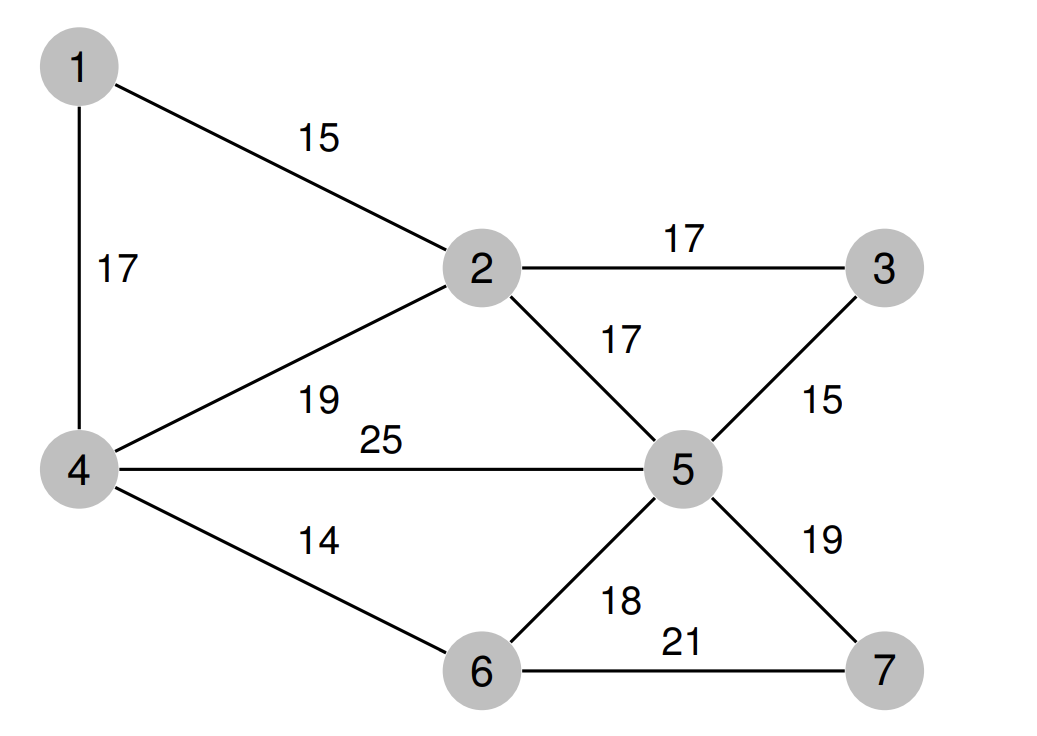
\includegraphics[scale=0.5]{estáticos/figura6.png}
\end{figure}
El algoritmo de Prim es un algoritmo perteneciente a la teoría de los grafos para encontrar un árbol recubridor mínimo en un grafo conexo, no dirigido y cuyas aristas están etiquetadas.

En otras palabras, el algoritmo encuentra un subconjunto de aristas que forman un árbol con todos los vértices, donde el peso total de todas las aristas en el árbol es el mínimo posible. Si el grafo no es conexo, entonces el algoritmo encontrará el árbol recubridor mínimo para uno de los componentes conexos que forman dicho grafo no conexo.

En este caso se utiliza de la siguiente manera:
\begin{enumerate}
    \item Parte desde el vértice 6,
    \item Selecciona la arista de menor peso que conecta el árbol con un vértice no incluido en el árbol. Selecciona la arista que une al 6 con el 4,
    \item Selecciona la arista de menor peso que conecta el árbol con un vértice no incluido en el árbol. Selecciona la arista que une al 4 con el 1,
    \item  Selecciona la arista de menor peso que conecta el árbol con un vértice no incluido en el árbol. Selecciona la arista que une al 1 con el 2,
    \item  Selecciona la arista de menor peso que conecta el árbol con un vértice no incluido en el árbol. Selecciona la arista que une al 2 con el 5,
    \item  Selecciona la arista de menor peso que conecta el árbol con un vértice no incluido en el árbol. Selecciona la arista que une al 5 con el 3.
    \item  Selecciona la arista de menor peso que conecta el árbol con un vértice no incluido en el árbol. Selecciona la arista que une al 5 con el 7.
\end{enumerate}

\begin{figure}[h]
    \centering
    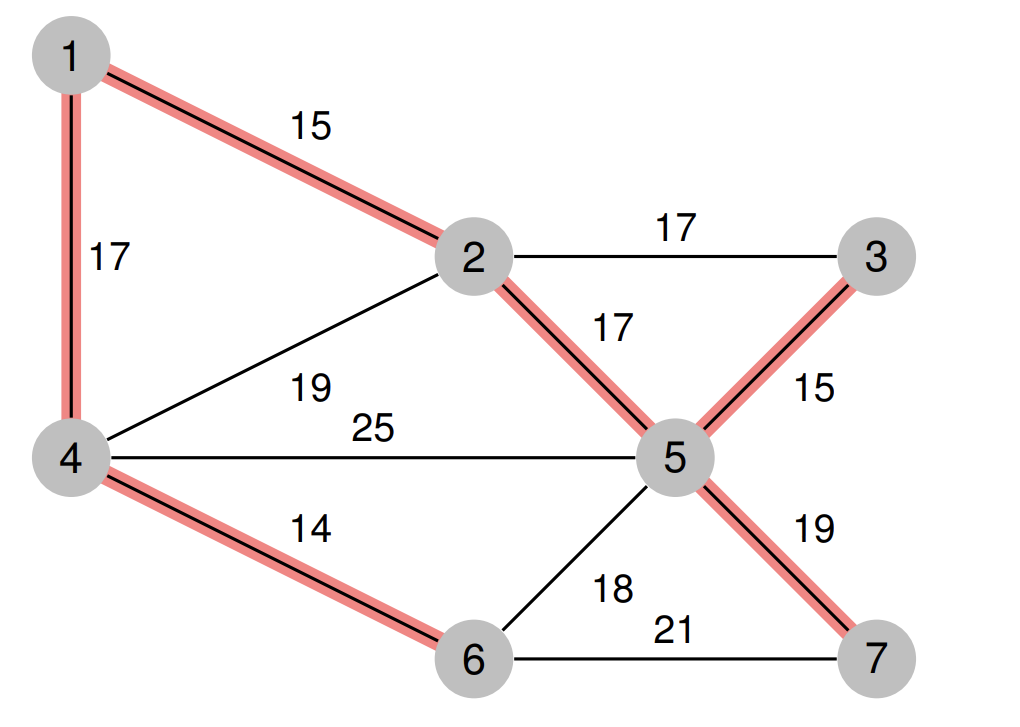
\includegraphics[scale=0.5]{estáticos/figura7.png}
\end{figure}

\begin{codebox}{Algoritmo de Prim}
\begin{pascallike}
type Vertex = Nat

type Edge = tuple
                v1 : Vertex
                v2 : Vertex
                cost : Nat
            end tuple

type Graph = tuple
                vertices : Set of Vertex
                edges : Set of Edge
            end tuple

fun Prim(G : Graph, k: Vertex) ret T: Set of Edge
    var c: Edge
    var C: Set of Vertex
    C:= copy_set(G.vertices)
    elim(C,k)
    T:= empty_set()
    do (not is\_empty\_set(C)) $\rightarrow$
        c := seleccionarArista(G.edges,C)
        if member(c.v1,C) then 
            elim(C,c.v1)
        else elim(C,c.v2)
        add(T,c)
        fi
    od
end fun
\end{pascallike}
\end{codebox}

\subsection{Camino de costo mínimo}

\begin{itemize}
    \item Se tiene un grafo conexo con pesos en las aristas.
    \item Se busca un camino que una dos vértices y cuya suma de pesos de las aristas sea mínima.
\end{itemize}

\subsubsection{Dijkstra}
El algoritmo de Dijkstra, también llamado algoritmo de caminos mínimos, es un algoritmo para la determinación del camino más corto, dado un vértice origen, hacia el resto de los vértices en un grafo que tiene pesos en cada arista. Su nombre alude a Edsger Dijkstra, científico de la computación de los Países Bajos que lo describió por primera vez en 1959.

La idea subyacente en este algoritmo consiste en ir explorando todos los caminos más cortos que parten del vértice origen y que llevan a todos los demás vértices; cuando se obtiene el camino más corto desde el vértice origen hasta el resto de los vértices que componen el grafo, el algoritmo se detiene. Se trata de una especialización de la búsqueda de costo uniforme y, como tal, no funciona en grafos con aristas de coste negativo (al elegir siempre el nodo con distancia menor, pueden quedar excluidos de la búsqueda nodos que en próximas iteraciones bajarían el costo general del camino al pasar por una arista con costo negativo).

Suponga que se tiene el siguiente grafo y se busca el camino de costo mínimo.
\begin{figure}[h]
    \centering
    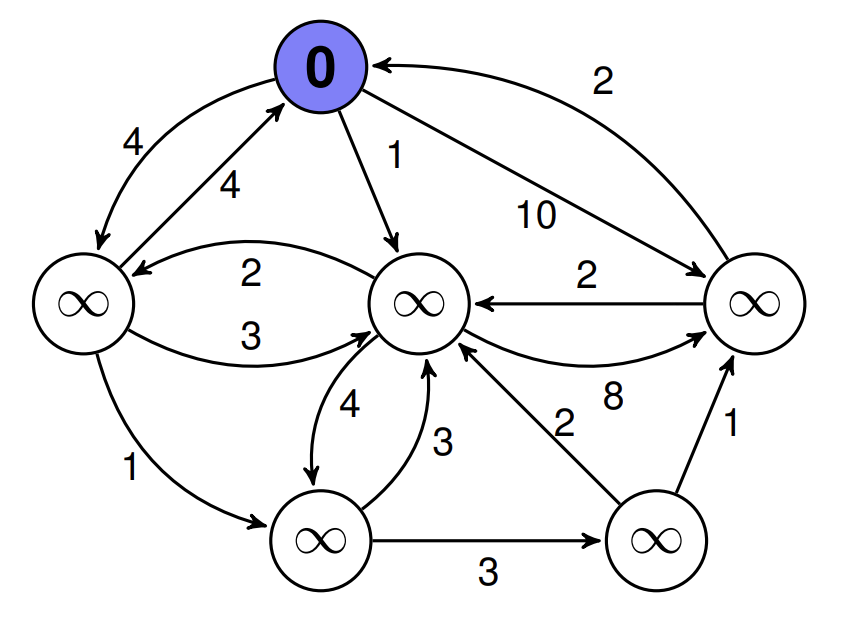
\includegraphics[scale=0.5]{estáticos/figura8.png}
\end{figure}

\begin{enumerate}
    \item Parte desde el vértice seleccionado, y actualiza los valores de los vértices adyacentes, y selecciona el de menor costo. La seleccion va $(0,1)$
    \item  Actualiza los valores de los vértices adyacentes, y selecciona el de menor costo $(0,1,3)$,
    \item  Actualiza los valores de los vértices adyacentes, y selecciona el de menor costo $(0,1,3,4)$,
    \item  Actualiza los valores de los vértices adyacentes, y selecciona el de menor costo $(0,1,3,4,7)$,
    \item  Actualiza los valores de los vértices adyacentes, y selecciona el de menor costo $(0,1,3,4,7,8)$,
    \item El algoritmo termina. No hay más vértices por visitar.
\end{enumerate}
\newpage
\begin{figure}[h]
    \centering
    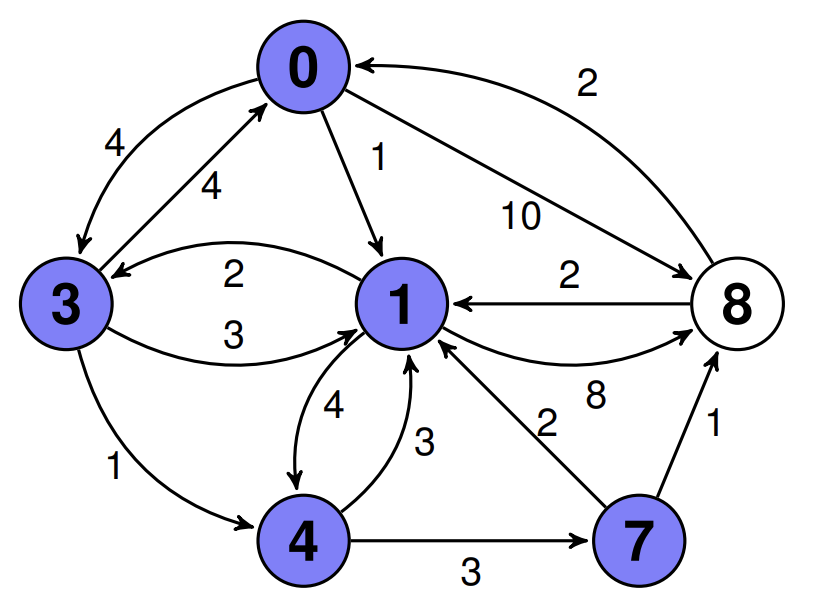
\includegraphics[scale=0.5]{estáticos/figura9.png}
\end{figure}

\begin{codebox}{Algoritmo de Dijkstra}
\begin{pascallike}
fun Dijkstra(L: array[1..n,1..n] of Nat, v: Nat) ret D: array[1..n] of Nat
    var c: Nat
    var C: Set of Nat
    for i := 1 to n do add(C,i) od
    elim(C,v)
    for j:= 1 to n do D[j]:= L[v,j] od
    do (not is_empty_set(C)) $\rightarrow$
        c:= seleccion(C,D)
        elim(C,c)
        for j in C do D[j]:= min(D[j],D[c]+L[c,j]) od
    od
end fun
\end{pascallike}
\end{codebox}

\begin{itemize}
    \item Se inicializa un conjunto $C$ con todos los vértices del grafo, excepto el vértice origen.
    \item Se inicializa un arreglo $D$ con las distancias desde el vértice origen a cada uno de los vértices del grafo.
    \item Se selecciona el vértice $c$ tal que $D[c]$ sea mínimo.
    \item Se elimina el vértice $c$ del conjunto $C$.
    \item Se actualizan las distancias de los vértices adyacentes a $c$.
    \item Se repiten los pasos anteriores hasta que el conjunto $C$ sea vacío.
\end{itemize}
    
\chapter{Backtracking (Vuelta Atrás - Fuerza Bruta)}

\section{Introducción}

El backtracking es una técnica de programación que se utiliza para encontrar soluciones a problemas computacionales. Se basa en la idea de que si se llega a un punto en el que no se puede continuar avanzando, se debe retroceder y probar otra opción. Es decir, se trata de un algoritmo recursivo que busca soluciones de manera sistemática, explorando todas las posibilidades hasta encontrar la correcta. 

Para hacer la conexión con algoritmos voraces, podríamos decir que no siempre un criterio voraz es suficiente para encontrar la solución óptima. En estos casos, el backtracking es una buena alternativa, ya que explora todas las posibilidades y encuentra la solución óptima. Con la desventaja de que es un algoritmo más costoso en términos de tiempo de ejecución.

\section{Estructura}
Normalmente se busca primero definir la función recursiva que resuelve el problema y luego se llama a esta función con los parámetros iniciales. La función recursiva se encarga de explorar todas las posibilidades, y en cada paso se verifica si se ha llegado a una solución o si se ha llegado a un punto en el que no se puede continuar avanzando. En este último caso, se retrocede y se prueba con otra opción.

\section{Ejemplo}
Retomando el problema de las monedas que vimos en el capítulo de algoritmos voraces, podemos ver que en algunos casos un algoritmo voraz no es suficiente para encontrar la solución óptima. Ahora vamos a hacer una versión de este problema utilizando backtracking.

La función recursiva es la siguiente:
$$
cambio(i, j) = 
\begin{cases}
    0 & j = 0 \\
    \infty & j > 0 \wedge i = 0 \\
    cambio(i - 1, j) &  d_i > j > 0 \wedge i > 0 \\
    min(cambio(i - 1, j), 1 + cambio(i, j - d_i)) & j \geq di > 0 \wedge i > 0
\end{cases}
$$
Que luego, se puede implementar en un lenguaje de programación de la siguiente manera:

\begin{codebox}{Problema del cambio de monedas con backtracking}
\begin{pascallike}
fun cambio(d:array[1..n] of nat, i,j: nat) ret r: nat
    if j=0 then r:= 0
    else if i = 0 then r:= $\infty$
    else if d[i] > j then r:= cambio(d,i-1,j)
    else r:= min(cambio(d,i-1,j),1+cambio(d,i,j-d[i]))
    fi
    r := cambio(d,n,j)
end fun    
\end{pascallike}
\end{codebox}

\subsection{Observaciones}

Cuando definimos de forma matemática la solución del problema, se siguen los siguientes estándares:
\begin{itemize}
    \item El conjunto de soluciones se expresa en tuplas, donde cada una es el valor de la solución.
    $$
    s = (v_1, v_2, \ldots, v_n)
    $$
    \item El conjunto parcial de soluciones será aquel en que se encuentre en cierto nivel K:
    $$
    s_p = (v_1, v_2,...,v_k) \\ \text{si } k ...
    $$
    \item Si se puede añadir un elemento más, la solución avanza a otro nivel $(K+1)$.
    \item Si no existe ningún valor, se retrocede al valor $(K-1)$.
    \item Se continua hasta que una solución parcial sea una solución al problema o hasta que no queden mas posibilidades a probar.
\end{itemize}

El resultado es equivalente a hacer una búsqueda en profundidad en el árbol de soluciones. Sin embargo, este árbol es implícito, no se almacena en ningún lugar.
\chapter{Programación Dinámica}

\section{Introducción}

La programación dinámica es una técnica de programación que se utiliza para resolver problemas computacionales. Se basa en la idea de descomponer un problema en subproblemas más pequeños y resolverlos de manera recursiva. Luego, se almacenan los resultados de los subproblemas para evitar tener que volver a calcularlos en el futuro. De esta forma, se reduce la complejidad del problema original y se obtiene una solución más eficiente.

Podríamos decir que la programación dinámica es una generalización de la técnica de divide y vencerás, ya que también se basa en la idea de descomponer un problema en subproblemas más pequeños. Sin embargo, a diferencia de divide y vencerás, la programación dinámica se utiliza cuando los subproblemas se solapan, es decir, comparten soluciones parciales. En estos casos, la programación dinámica es más eficiente, ya que evita tener que resolver los mismos subproblemas varias veces. Cuando trabajamos con soluciones con backtracking, cabe destacar que la programación dinámica viene a ser una mejora de esta técnica, ya que evita tener que recalcular los mismos subproblemas.

\section{Problema de la mochila para explicar la programación dinámica}
¿Qué objetos deberías robar para obtener el mayor valor posible en dinero?

\begin{figure}[h]
    \centering
    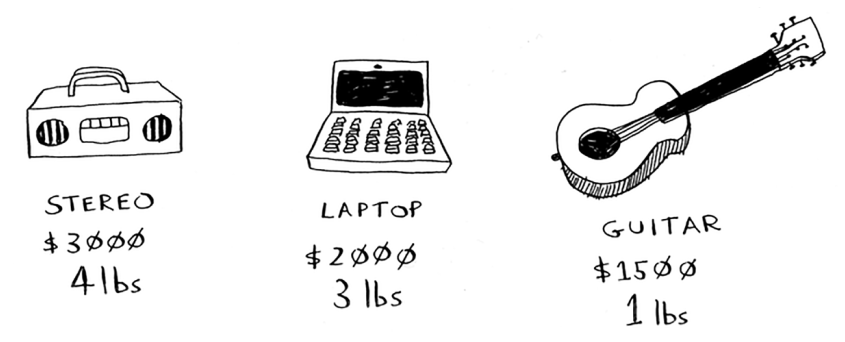
\includegraphics[width=0.7\textwidth]{estáticos/figura11.png}
    \caption{Problema de la mochila}
\end{figure}

El algoritmo más simple es este: probas con cada conjunto posible de objetos y encuentras el conjunto que te da el mayor valor.

\begin{figure}[h]
    \centering
    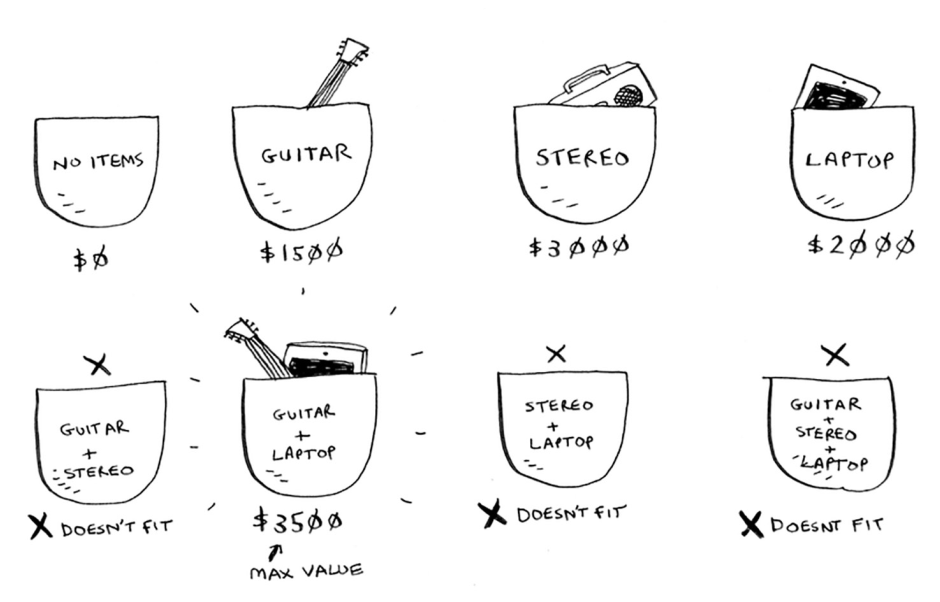
\includegraphics[width=0.6\textwidth]{estáticos/figura12.png}
    \caption{Algoritmo de fuerza bruta para el problema de la mochila}
\end{figure}

Esto funciona, pero es realmente lento. Para 3 objetos, hay que calcular 8 conjuntos posibles. Para 4 objetos, calcular 16 conjuntos. Con cada objeto que agregas el número de conjuntos que tienes que calcular se duplica. Este algoritmo toma un tiempo de O($2^n$), lo cual es muy, muy lento y es el visto anteriormente como \textit{backtracking}.

\newpage
\textbf{¿Cómo podemos hacerlo más rápido?} Con \textit{programación dinámica}, comienza resolviendo subproblemas y se va construyendo hasta resolver el problema principal. Para el problema de la mochila, comienza resolviendo el problema para mochilas más pequeñas (o “sub-mochilas”) y luego trabajar hasta resolver el problema original.

\begin{figure}[h]
    \centering
    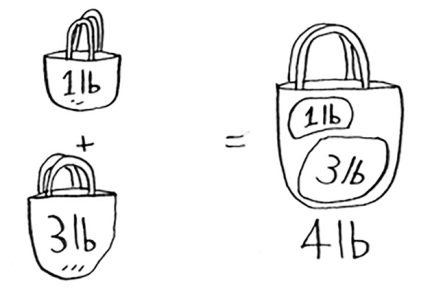
\includegraphics[width=0.4\textwidth]{estáticos/figura13.png}
    \caption{Algoritmo de programación dinámica para el problema de la mochila}
\end{figure}

¿En que se basa la programación dinámica que lo hace más rápido? En lugar de calcular el valor de cada conjunto posible de objetos, se calcula el valor de cada objeto en cada capacidad de mochila posible. Luego, se usa esa información para calcular el valor de los objetos en una mochila de mayor capacidad. De esta forma, se evita tener que recalcular los mismos subproblemas una y otra vez. Todo problema de programación dinámica comienza con una tabla, en este caso puede ser de esta forma:

\newpage
\begin{figure}[h]
    \centering
    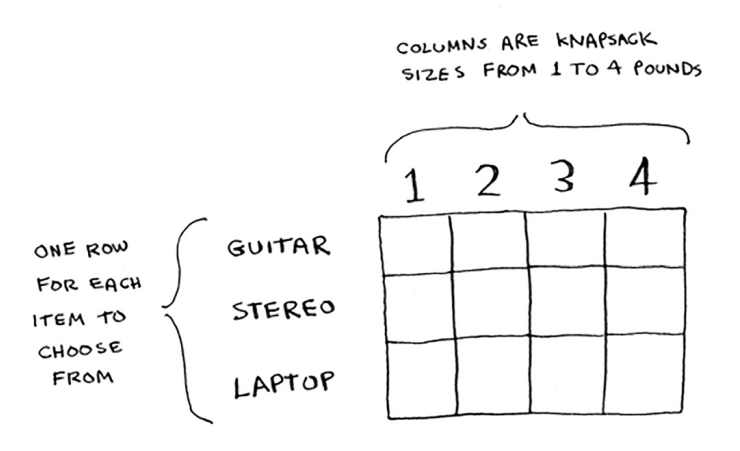
\includegraphics[width=0.65\textwidth]{estáticos/figura14.png}
    \caption{Tabla de programación dinámica para el problema de la mochila}
\end{figure}

Las filas de la cuadrícula son los objetos, y las columnas son los pesos de la mochila desde 1 lb hasta 4 lb. Necesitas todas esas columnas porque te ayudarán a calcular los valores de las sub-mochilas. La cuadrícula comienza vacía. Se va a llenar cada celda de la cuadrícula. Una vez que la cuadrícula esté llena, se tiene la respuesta al problema final.

Cuando te posiciones la fila de la guitarra, lo que significa que estás tratando de meter la guitarra en la mochila. En cada celda, hay una decisión simple: ¿Colocas la guitarra o no? Recuerda, estás tratando de encontrar el conjunto de objetos a robar que te dará el mayor valor.
La primera celda tiene una mochila con una capacidad de 1 lb. La guitarra también pesa 1 lb, ¡lo que significa que cabe en la mochila! Entonces, el valor de esta celda es \$1,500, y contiene una guitarra. Así se llenaria la tabla completa de esta forma:

\begin{figure}[h]
    \centering
    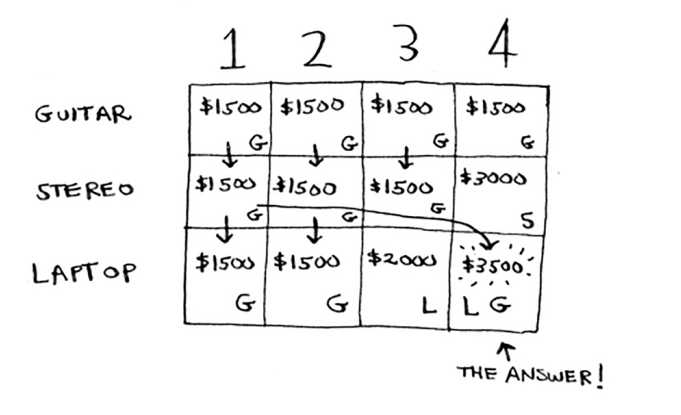
\includegraphics[width=0.45\textwidth]{estáticos/figura15.png}
    \caption{Tabla de programación dinámica para el problema de la mochila}
\end{figure}

Para calcular las demas celdas, el criterio es el siguiente: si el objeto cabe en la mochila, se calcula el valor de la mochila sin el objeto y se le suma el valor del objeto. Si el objeto no cabe en la mochila, se copia el valor de la celda de arriba. De esta forma, se va llenando la tabla hasta que se llega a la celda de la esquina inferior derecha, que contiene el valor de la mochila con todos los objetos.


\newpage
\section{Programación dinámica formalmente en el lenguaje de la materia}
Veamos por ejemplo el problema de la moneda:

\begin{codebox}{Problema del cambio de monedas con programación dinámica}
\begin{pascallike}
fun cambio(d:array[1..n] of nat, k: nat) ret r: nat
    var cam: array[0..n,0..k] of nat
    for i:= 0 to n do cam[i,0]:= 0 od
    for j:= 1 to k do cam[0,j]:= $\infty$ od
    for i:= 1 to n do
        for j:= 1 to k do
            if d[i] > j then cam[i,j]:= cam[i-1,j]
            else cam[i,j]:= min(cam[i-1,j],1+cam[i,j-d[i]])
            fi
        od
    od
    r:= cam[n,k]
end fun
\end{pascallike}
\end{codebox}

Así podemos ver la tabla de la solución del problema de las monedas:

\begin{figure}[h]
    \centering
    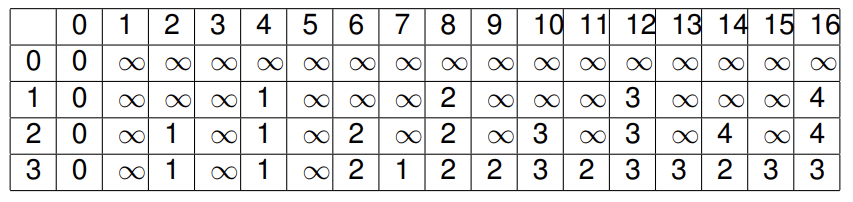
\includegraphics[width=0.8\textwidth]{estáticos/figura10.png}
    \caption{Tabla de programación dinámica para el problema del cambio de monedas}
\end{figure}

\subsection{Observaciones}

Siempre los problemas tienen la siguiente estructura:
\begin{itemize}
    \item Casos base: son los casos más simples y fáciles de resolver.
    \item Subproblemas: son los problemas más pequeños en los que se descompone el problema original.
    \item Soluciones parciales: son los resultados de los subproblemas.
    \item Solución final: es la solución al problema original, que se obtiene a partir de las soluciones parciales. Suele ser una llamada principal dependiendo de cuales son los parámetros de entrada.
\end{itemize}
Otras observaciones:
\begin{enumerate}
    \item Puedes usar programación dinámica cuando el problema se puede dividir en subproblemas discretos.
    \item Cada solución de programación dinámica implica una cuadrícula.
    \item Los valores en las celdas son generalmente lo que estás tratando de optimizar.
    \item Cada celda es un subproblema, así que piensa en cómo puedes dividir tu problema en subproblemas.
    \item No hay una fórmula única para calcular una solución de programación dinámica.
\end{enumerate}

\chapter{Ejercicios Resueltos}

\section{Ordenación elemental}
Escribí algoritmos para resolver cada uno de los siguientes problemas sobre un arreglo a de posiciones $1$ a $n$, utilizando do. Elegí en cada caso entre estos dos encabezados el que sea más adecuado:

\begin{codebox}{Ejercicio 1}
\begin{pascallike}
proc nombre (in/out a: array [1..n] of nat)
    ...
end proc
\end{pascallike}
\end{codebox}
\begin{codebox}{Ejercicio 1}
\begin{pascallike}
proc nombre (out a: array [1..n] of nat)
    ...
end proc
\end{pascallike}
\end{codebox}
\begin{itemize}
    \item[(a)] Inicializar cada componente del arreglo con el valor $0$.
    \item[(b)] Inicializar el arreglo con los primeros $n$ números naturales positivos.
    \item[(c)] Inicializar el arreglo con los primeros $n$ números naturales impares.
    \item[(d)] Incrementar las posiciones impares del arreglo y dejar intactas las posiciones pares.  
\end{itemize}

\begin{codebox}{Solución (a)}
\begin{pascallike}
proc inicializarConCero (out a: array [1..n] of nat)
    i := 1
    do i <= n -> 
    a[i] := 0
    i := i + 1
    od
end proc
\end{pascallike}
\end{codebox}
\begin{codebox}{Solución (b)}
\begin{pascallike}
proc inicializarConNaturales (out a: array [1..n] of nat)
    i := 1
    do i <= n -> 
    a[i] := i
    i := i + 1
    od
end proc
\end{pascallike}
\end{codebox}
\begin{codebox}{Solución (c)}
\begin{pascallike}
proc inicializarConImpares (out a: array [1..n] of nat)
    i := 1
    do i <= n -> 
    a[i] := 2 * i - 1
    i := i + 1
    od
end proc
\end{pascallike}
\end{codebox}
\begin{codebox}{Solución (d)}
\begin{pascallike}
proc incrementarImpares (in/out a: array [1..n] of nat)
    i := 1
    do i <= n -> 
    if i mod 2 = 1 then
        a[i] := a[i] + 1
    fi
    i := i + 1
    od
end proc
\end{pascallike}
\end{codebox}

\begin{center}
    \rule{\textwidth}{0.4pt}
\end{center}

Escribí un algoritmo que reciba un arreglo a de posiciones 1 a n y determine si el arreglo recibido está ordenado o no. Explicá en palabras \textbf{qué} hace el algoritmo. Explicá en palabras \textbf{cómo} lo hace.

\begin{codebox}{Solución}
\begin{pascallike}
fun estaOrdenado (a: array [1..n] of nat) ret r: bool
    r := true
    for i := 1 to n - 1 do
    if a[i] > a[i + 1] then
        r := false
    else
        skip
    fi
    od
end fun
\end{pascallike}
\end{codebox}

\begin{center}
    \rule{\textwidth}{0.4pt}
\end{center}
\newpage
Ordená los siguientes arreglos, utilizando el algoritmo de ordenación por selección visto en clase. Mostrá en cada paso de iteración cuál es el elemento seleccionado y cómo queda el arreglo después de cada intercambio.

\begin{itemize}
    \item[(a)] $[7, 1, 10, 3, 4, 9, 5]$
\end{itemize}

\begin{figure}[h]
    \centering
    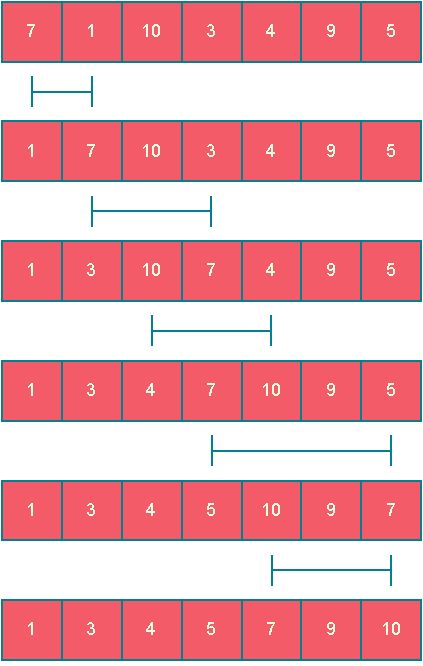
\includegraphics[scale=0.8]{estáticos/4a.pdf}
\end{figure}

\begin{center}
    \rule{\textwidth}{0.4pt}
\end{center}

Descifrá qué hacen los siguientes algoritmos, explicar cómo lo hacen y reescribirlos asignando nombres adecuados a todos los identificadores.

\begin{codebox}{Ejercicio 6 (a)}
\begin{pascallike}
proc p (in/out a: array [1..n] of T)
    var x: nat
    for i := n downto 2 do
    x := f(a,i)
    swap(a,i,x)
    od
end proc
\end{pascallike}
\end{codebox}

\begin{codebox}{Ejercicio 6 (b)}
\begin{pascallike}
fun f (a: array [1..n] of T, i: nat) ret x: nat
    x := 1
    for j := 2 to i do
    if a[j] > a[x] then
        x := j
    fi
    od
end fun
\end{pascallike}
\end{codebox}

\textbf{Algoritmo p:} El algoritmo recibe un arreglo de elementos de tipo T y lo ordena de manera descendente. Para ello, recorre el arreglo desde la última posición hasta la segunda, en cada iteración busca el elemento más grande en el subarreglo que va desde la primera posición hasta la posición actual y lo intercambia con el elemento en la posición actual.
Se podria escribir de la siguiente manera:

\begin{codebox}{Solución (a)}
\begin{pascallike}
proc ordenarDescendente (in/out a: array [1..n] of T)
    var posMax: nat
    for i := n downto 2 do
    posMax := buscarMaximo(a,i)
    swap(a,i,posMax)
    od
end proc
\end{pascallike}
\end{codebox}

\textbf{Función f:} La función recibe un arreglo de elementos de tipo T y un número natural $i$, y retorna la posición del elemento más grande en el subarreglo que va desde la primera posición hasta la posición $i$. Para ello, recorre el subarreglo desde la segunda posición hasta la posición $i$, en cada iteración compara el elemento actual con el elemento más grande encontrado hasta el momento y si el elemento actual es mayor, actualiza la posición del elemento más grande.
Se podria escribir de la siguiente manera:

\begin{codebox}{Solución (b)}
\begin{pascallike}
fun buscarMaximo (a: array [1..n] of T, i: nat) ret posMax: nat
    posMax := 1
    for j := 2 to i do
    if a[j] > a[posMax] then
        posMax := j
    fi
    od
end fun
\end{pascallike}
\end{codebox}

\section{Ordenación avanzada}

\begin{itemize}
    \item[a)] Escribí el procedimiento "\texttt{intercalar\_cada}" que recibe un arreglo $a : array[1..2^n] of int$ y un número natural $i : nat$; e intercala el segmento $a[1, 2^i]$ con $a[2^i + 1, 2 * 2^i]$, el segmento $a[2 * 2^i + 1, 3 * 2^i]$ con $a[3 * 2^i + 1, 4 * 2^i]$, etc. Cada uno de dichos segmentos se asumen ordenados. Por ejemplo, si el arreglo contiene los valores $3, 7, 1, 6, 1, 5, 3, 4$ y se lo invoca con con $i = 1$ el algoritmo deberá devolver el arreglo $1, 3, 6, 7, 1, 3, 4, 5$. Si se lo vuelve a invocar con este nuevo arreglo y con $i = 2$, devolverá $1, 1, 3, 3, 4, 5, 6, 7$ que ya está completamente ordenado. El algoritmo asume que cada uno de estos segmentos está ordenado, y puede utilizar el procedimiento de intercalación dado en clase
    \item[b)] Utilizar el algoritmo "\texttt{intercalar\_cada}" para escribir una versión iterativa del algoritmo de ordenación por intercalación. La idea es que en vez de utilizar recursión, invoca al algoritmo del inciso anterior sucesivamente con $i = 0, 1, 2, 3,$ etc.
\end{itemize}

Primero para definir el procedimiento, va a recibir un arreglo \texttt{a : array[1..$2^n$] of int} y un número natural $i : nat$:

\begin{codebox}{Estructura}
\begin{pascallike}
proc intercalar_cada(in/out a: array[1..$2^n$] of Int, in i: nat)
...
end proc
\end{pascallike}
\end{codebox}
para poder intercalar el arreglo, se va a tener que llamar a la función \texttt{merge}, que toma un arreglo, y 3 posiciones \texttt{lft}, \texttt{mid}, \texttt{rgt}. Entonces hay que definirlas:

\begin{codebox}{Inicialización de variables}
\begin{pascallike}
proc intercalar_cada(in/out a: array[1..$2^n$] of Int, in i: nat)
    var lft, rgt, mid: nat
    ...
end proc
\end{pascallike}
\end{codebox}
Se deberia agregar una variable natural para recorrer cada segmento del arreglo

\begin{codebox}{Inicialización de variables}
\begin{pascallike}
proc intercalar_cada(in/out a: array[1..$2^n$] of Int, in i: nat)
    var lft, rgt, mid: nat {-Variables para llamar a merge-}
    var k: nat {-Variable para recorrer el arreglo-}
    ...
end proc
\end{pascallike}
\end{codebox}
La idea principal es realizar la intercalación de segmentos del arreglo según el valor proporcionado \texttt{i}, cada segmento tiene un tamaño de $2^i$ elementos. Para ello se debe hacer un ciclo while que calcule cada uno de los índices para llamar a la función de intercalación.

\begin{codebox}{Ciclo while}
\begin{pascallike}
proc intercalar_cada(in/out a: array[1..$2^n$] of Int, in i: nat)
    var lft, rgt, mid: nat {-Variables para llamar a merge-}
    var k: nat {-Variable para recorrer el arreglo-}
    while k $\leq$ $2^n$ do
    lft := ... {-Indice inicial del primer segmento-}
    mid := ... {-Indice final del primer segmento-}
    rgt := ... {-Indice final del segundo segmento-}
    merge(a,lft,mid,rgt) {-Llamada a la funcion para intercalar-}
    k := ...
    do
end proc
\end{pascallike}
\end{codebox}
El índice lft será primero $1$, siguiendo la estructura de los segmentos, deberia tomar el valor de $k * 2^i + 1$, luego el medio es $(j+1) * 2^i$ y el final es $(j+2) * 2^i$.
\begin{codebox}{Procedimiento completo}
\begin{pascallike}
proc intercalar_cada(in/out a: array[1..$2^n$] of Int, in i: nat)
    var lft, rgt, mid: nat {-Variables para llamar a merge-}
    var k: nat {-Variable para recorrer el arreglo-}
    while k $\leq$ $2^n$ do
    lft := k * $2^i$ + 1 {-Indice inicial del primer segmento-}
    mid := (k+1) * $2^i$ {-Indice final del primer segmento-}
    rgt := (k+2) * $2^i$ {-Indice final del segundo segmento-}
    merge(a,lft,mid,rgt) {-Llamada a la funcion para intercalar-}
    k := k+2
    do
end proc
\end{pascallike}
\end{codebox}
\begin{codebox}{Solución}
\begin{pascallike}
proc intercalar_cada_iter (in/out array[1..$2^n$] of int)
    for i := 0 to n-1 do
    intercalar_cada(a,i)
    od
end proc
\end{pascallike}
\end{codebox}

\begin{center}
    \rule{\textwidth}{0.4pt}
\end{center}

Escribí un algoritmo que dado un arreglo \texttt{a : array[1..n] of int} y un número natural $k \leq n$ devuelve el elemento de \texttt{a} que quedaría en la celda \texttt{a[k]} si a estuviera ordenado. Está permitido realizar intercambios en \texttt{a}, pero no ordenarlo totalmente. La idea es explotar el hecho de que el procedimiento partition del quick sort deja al pivot en su lugar correcto.

\begin{codebox}{Algoritmo}
\begin{pascallike}
fun encontrarElemento(a: array[1..n] of int, k: nat): ret r : int
    var lft, rgt, ppiv: nat

    lft := 1
    rgt := n

    do lft < rgt -->
        partition(a, lft, rgt, ppiv)

        if ppiv = k -->
            r := a[ppiv]
        [] ppiv < k -->
            lft := ppiv + 1
        [] -->
            rgt := ppiv - 1
        fi
    od

    r := a[k]
end proc
\end{pascallike}
\end{codebox}

\begin{center}
    \rule{\textwidth}{0.4pt}
\end{center}

El procedimiento \texttt{partition} que se dio en clase separa un fragmento de arreglo principalmente en dos segmentos: menores o iguales al pivot por un lado y mayores o iguales al pivot por el otro. Modificá ese algoritmo para que separe en tres segmentos: los menores al pivot, los iguales al pivot y los mayores al pivot. En vez de devolver solamente la variable \texttt{pivot}, deberá devolver \texttt{pivot izq} y \texttt{pivot} der que informan al algoritmo \texttt{quick\_sort\_rec} las posiciones inicial y final del segmento de repeticiones del \texttt{pivot}. Modificá el algoritmo \texttt{quick\_sort\_rec} para adecuarlo al nuevo procedimiento \texttt{partition}.

\textbf{Procedimiento \texttt{partition} modificado:}

\begin{codebox}{Partition modificado}
\begin{pascallike}
proc partition(in/out a: array[1..n] of T, in lft, rgt: nat, 
out pivotIzq, pivotDer: nat)
    var i, j, pivotPos: nat
    {-pivotPos rastrea la posicion actual del pivote-}
    pivotPos := lft
    i := lft + 1
    j := rgt

    do i <= j -->
        {-Casos para manejar elementos menores, mayores e iguales al pivote-}
        if a[i] < a[pivotPos] -->
            i := i + 1
        [] a[j] > a[pivotPos] -->
            j := j - 1
        [] a[i] > a[pivotPos] -->
            swap(a, i, j)
        {-Caso para manejar repeticiones del pivote-}
        [] -->
            swap(a, i, pivotPos)
            pivotPos := i
            i := i + 1
            j := j - 1
        fi
    od
    {-pivotIzq es la posicion inicial del segmento de repeticiones del pivote-}
    pivotIzq := lft
    {-pivotDer es la posicion final del segmento de repeticiones del pivote-}
    pivotDer := j
    {-Mover todas las repeticiones del pivote a posiciones contiguas despues 
    de pivotIzq-}
    do j < rgt -->
        swap(a, j + 1, rgt)
        j := j + 1
    od
end proc

proc quick_sort_rec(in/out a: array[1..n] of T, in lft, rgt: nat)
    var pivotIzq, pivotDer: nat

    if lft < rgt -->
        partition(a, lft, rgt, pivotIzq, pivotDer)
        quick_sort_rec(a, lft, pivotIzq - 1)
        quick_sort_rec(a, pivotDer + 1, rgt)
    fi
end proc
\end{pascallike}
\end{codebox}

\section{Recurrencia Divide y Vencerás}

Calculá el orden de complejidad de los siguientes algoritmos:

\begin{codebox}{(a)}
\begin{pascallike}
proc f1(in n : nat)
    if n $\leq$ 1 then skip
    else
        for i := 1 to 8 do 
            f1(n div 2) 
        od
        for i := 1 to $n^3$ do 
            t := 1 
        od
    fi
end proc
\end{pascallike}
\end{codebox}

\begin{codebox}{(b)}
\begin{pascallike}
proc f2(in n : nat)
    for i := 1 to n do
        for j := 1 to i do 
            t := 1 
        od
    od
    if n > 0 then
        for i := 1 to 4 do 
            f2(n div 2) 
        od
    fi
end proc
\end{pascallike}
\end{codebox}

\textbf{Solución (a)}
En este caso notar que:
\begin{itemize}
    \item Tamaño de la entrada: $n$,
    \item Operación a contar: $t := 1$.
\end{itemize}
Entonces, se puede definir una funcion $r(n)$, que representará la cantidad de asignaciones a la variable $t$ que ocurren al llamar a la función $f1$ con el dato de entrada $n$.

Podemos observar que la función $f1$ esta dividida en dos casos, si $n \leq 1$ entonces no se realiza ninguna asignación a la variable $t$, por lo que $r(n) = 0$.
\begin{equation*}
    r(n) = 
    \begin{cases}
        0 & \text{si } n \leq 1 \\
        ... & \text{en caso contrario}
    \end{cases}
\end{equation*}
Como hay dos ciclos for en una secuencia, se puede analizar cada uno por separado y sumarlos, por ahora los puedo expresar como sumatoria:
\begin{equation*}
    r(n) = 
    \begin{cases}
        0 & \text{si } n \leq 1 \\
        \sum_{i=1}^{8} ... + \sum_{i=1}^{n^3} ... & \text{en caso contrario}
    \end{cases}
\end{equation*}
En el primer for, queremos contar la cantidad de asignaciones que se realizan al llamar a la función $f1$ con el dato de entrada $n/2$, por lo que se puede expresar como:
\begin{equation*}
    r(n) = 
    \begin{cases}
        0 & \text{si } n \leq 1 \\
        \sum_{i=1}^{8} r(n/2) + \sum_{i=1}^{n^3} ... & \text{en caso contrario}
    \end{cases}
\end{equation*}
En el segundo for, se realiza una asignación a la variable $t$ por cada iteración, por lo que se puede expresar como:
\begin{equation*}
    r(n) = 
    \begin{cases}
        0 & \text{si } n \leq 1 \\
        \sum_{i=1}^{8} r(n/2) + \sum_{i=1}^{n^3} 1 & \text{en caso contrario}
    \end{cases}
\end{equation*}
Resolviendo las sumatorias, se obtiene:
\begin{equation*}
    r(n) = 
    \begin{cases}
        0 & \text{si } n \leq 1 \\
        8 \cdot r(n/2) + n^3 & \text{en caso contrario}
    \end{cases}
\end{equation*}
Por lo que se puede observar que:
\begin{itemize}
    \item $a = 8$,
    \item $b = 2$,
    \item $g(n) = n^3$.
\end{itemize}
Como $a = 8 = 2^3 = b^3$, se puede decir que el orden de complejidad es $O(n^3 \log n)$.

\textbf{Solución (b)}
En este caso notar que:
\begin{itemize}
    \item Tamaño de la entrada: $n$,
    \item Operación a contar: $t := 1$.
\end{itemize}
Entonces, se puede definir una funcion $r(n)$, que representará la cantidad de asignaciones a la variable $t$ que ocurren al llamar a la función $f2$ con el dato de entrada $n$.

En este caso la función $f2$ está dividida en $n$ casos (cada uno representado por el valor de $i$):
\begin{equation*}
    r(n) = 
    \begin{cases}
        \sum_{i=1}^{n} \sum_{j=1}^{i} 1 & \text{casos simples }  \\
        ... & \text{en caso contrario}
    \end{cases}
\end{equation*}
En el for dentro del if, se realiza una llamada recursiva a la función $f2$ con el dato de entrada $n/2$, por lo que se puede expresar como:
\begin{equation*}
    r(n) = 
    \begin{cases}
        \sum_{i=1}^{n} \sum_{j=1}^{i} 1 & \text{casos simples }  \\
        \sum_{i=1}^{n} \sum_{j=1}^{i} 1 +  \sum_{i=1}^{4} r(n/2) & \text{en caso contrario}
    \end{cases}
\end{equation*}
Resolviendo las sumatorias, se obtiene:
\begin{equation*}
    r(n) = 
    \begin{cases}
        \sum_{i=1}^{n} i & \text{casos simples }  \\
        \sum_{i=1}^{n} i +  \sum_{i=1}^{4} r(n/2) & \text{en caso contrario}
    \end{cases}
\end{equation*}
\begin{equation*}
    r(n) = 
    \begin{cases}
        \frac{n\cdot (n+1)}{2} & \text{casos simples }  \\
        \frac{n\cdot (n+1)}{2} + 4 \cdot r(n/2) & \text{en caso contrario}
    \end{cases}
\end{equation*}

Por lo que se puede observar que:
\begin{itemize}
    \item $a = 4$,
    \item $b = 2$,
    \item $g(n) = \frac{n\cdot (n+1)}{2}$.
\end{itemize}
Como $a = 4 = 2^2 = b^2$, se puede decir que el orden de complejidad es $O(n^2 \log n)$.

\begin{center}
    \rule{\textwidth}{0.4pt}
\end{center}

Dado un arreglo \texttt{a : array[1..n] of nat} se define una cima de $a$ como un valor $k$ en el intervalo $1, . . . ,n$ tal que $a[1..k]$ está ordenado crecientemente y $a[k..n]$ está ordenado decrecientemente.
\begin{itemize}
    \item[(a)] Escribá un algoritmo que determine si un arreglo dado tiene cima.
    \item[(b)] Escribí un algoritmo que encuentre la cima de un arreglo dado (asumiendo que efectivamente tiene una cima) utilizando una búsqueda secuencial, desde el comienzo del arreglo hacia el final. 
    \item[(c)] Escribí un algoritmo que resuelva el mismo problema del inciso anterior utilizando la idea de \texttt{búsqueda binaria}.
    \item[(d)] Calculá y compará el orden de complejidad de ambos algoritmos.
\end{itemize}

Para determinar si un arreglo tiene cima, se puede recorrer el arreglo y buscar el máximo que va a ser el probable punto cima.

\begin{codebox}{Estructura}
\begin{pascallike}
fun tieneCima (a : array[1..n] of nat) ret r : bool
    r := false
    var tempos : nat
    {-Busco la posible cima y lo guardo en tempos-}
    for i := 2 to n do
        if a[i-1] < a[i] then
            tempos := i
            r := true
        fi
    od
    ...
end fun
\end{pascallike}
\end{codebox}

Luego de encontrar un elemento, habria que verificar si el resto del arreglo cumple con la condición de cima.

\begin{codebox}{Solución final}
\begin{pascallike}
fun tieneCima (a : array[1..n] of nat) ret r : bool
    r := false
    var tempos : nat
    {-Busco la posible cima y lo guardo en tempos-}
    for i := 2 to n do
        if a[i-1] < a[i] then
            tempos := i
            r := true
        fi
    od
    {-Si hay alguna posible cima, verifico que el resto arreglo cumpla-}
    for i := 1 to tempos do
        if a[i] < a[i+1] then
            r := false
        fi
    od
    for i := tempos to n do
        if a[i] > a[i+1] then
            r := false
        fi
    od
end fun
\end{pascallike}
\end{codebox}

Para encontrar la cima y devolverla, el algoritmo es el mismo que el anterior con la diferencia de que en vez de devolver el valor de r, devuelvo el valor del arreglo en la posición tempos (y la verificación de si hay cima o no se puede omitir ya que se asume que hay cima).

\begin{codebox}{Solución final}
\begin{pascallike}
fun cima (a : array[1..n] of nat) ret c : nat
    var tempos : nat
    {-Busco la cima y lo guardo en tempos-}
    for i := 2 to n do
        if a[i-1] < a[i] then
            tempos := i
        fi
    od
    c := a[tempos]
end fun
\end{pascallike}
\end{codebox}

Para encontrar la cima y devolverla, se puede utilizar la idea de búsqueda binaria. Se puede buscar el punto cima de la siguiente manera:

\begin{itemize}
    \item Se toma el punto medio del arreglo y se compara con el siguiente elemento.
    \item Si el punto medio es menor al siguiente elemento, entonces la cima se encuentra en la mitad derecha del arreglo.
    \item Si el punto medio es mayor al siguiente elemento, entonces la cima se encuentra en la mitad izquierda del arreglo.
\end{itemize}

\begin{codebox}{Solución}
\begin{pascallike}
fun busqueda_binaria_rec (a : array[1..n] of nat, lft, rgt: nat) ret i : nat
var mid : nat
if lft < rgt then
    i := 0
else
    mid := (lft + rgt) div 2
    if a[mid-1] $\geq$ a[mid] $\wedge$ a[mid+1] $\geq$ a[mid] then
        i := busqueda_binaria_rec(a, lft, mid-1)
    fi
    if a[mid-1] $\leq$ a[mid] $\wedge$ a[mid+1] $\leq$ a[mid] then
        i := mid
    fi
    if a[mid-1] $\leq$ a[mid] $\wedge$ a[mid+1] $\geq$ a[mid] then
        i := busqueda_binaria_rec(a, mid+1, rgt)
    fi
fi
end fun

fun cima (a : array[1..n] of nat) ret c : nat
    c := busqueda_binaria_rec(a, 2, n-1)
end fun
\end{pascallike}
\end{codebox}

\textbf{Solución (d)}
Para el algoritmo de búsqueda secuencial, se puede observar que el peor caso es cuando la cima se encuentra en la última posición del arreglo, por lo que se recorre todo el arreglo. Por lo que el orden de complejidad es $O(n)$.

Para el algoritmo de búsqueda binaria, se puede observar que el peor caso es cuando la cima se encuentra en la mitad del arreglo, por lo que se divide el arreglo en dos partes y se busca en una de ellas. Por lo que el orden de complejidad es $O(\log n)$.

\newpage
\section{Tipos de datos concretos}

Escribir un algoritmo que dada una matriz \texttt{a: array[1..n,1..m] of int} calcule el elemento mínimo. Escribir otro algoritmo que devuelva un arreglo \texttt{array[1..n]} con el mínimo de cada fila de la matriz \texttt{a}.

\begin{codebox}{Ejercicio 1.1}
\begin{pascallike}
fun min_elem_array(a : array[1..n,1..m] of int) ret min_elem int
    min_elem := a[1][1];
    for fil:= 1 to n do
        for col:= 1 to m do
            if a[fil][col] < min_elem then
                min_elem := a[col][fil];
            fi
        od
    od
end fun
\end{pascallike}
\end{codebox}

\begin{codebox}{Ejercicio 1.2}
\begin{pascallike}
fun array_of_mins(a: array[1..n,1..m] of int) ret array_min array[1..n] of int
    for fil:= 1 to n do
        array_min[fil] := min_elem_array(a[fil, 1..m])
    od
end fun
\end{pascallike}
\end{codebox}

\begin{center}
    \rule{\textwidth}{0.4pt}
\end{center}

Dados los tipos enumerados

\begin{codebox}{mes}
\begin{pascallike}
type mes = enumerate
            enero
            febrero
            ...
            diciembre
           end enumerate
\end{pascallike}
\end{codebox}

\begin{codebox}{clima}
\begin{pascallike}
type clima = enumerate
                Temp
                TempMax
                TempMin
                Pres
                Hum
                Prec
             end enumerate
\end{pascallike}
\end{codebox}

El arreglo \texttt{med:array[1980..2016,enero..diciembre,1..28,Temp..Prec] of nat} es un arreglo multidimensional que contiene todas las mediciones estadísticas del clima para la ciudad de Córdoba desde el 1/1/1980 hasta el 28/12/2016. Por ejemplo, \texttt{med[2014,febrero,3,Pres]} indica la presión atmosférica que se registró el día 3 de febrero de 2014. Todas las mediciones están expresadas con números enteros. Por simplicidad asumiremos que todos los meses tienen 28 días.

\begin{itemize}
    \item[(a)] Dar un algoritmo que obtenga la menor temperatura mínima (TempMin) histórica registrada en la ciudad de Córdoba según los datos del arreglo.
    \item[(b)] Dar un algoritmo que devuelva un arreglo que registre para cada año entre 1980 y 2016 la mayor temperatura máxima (TempMax) registrada durante ese año.
    \item[(c)] Dar un algoritmo que devuelva un arreglo que registre para cada año entre 1980 y 2016 el mes de ese año en que se registró la mayor cantidad mensual de precipitaciones (Prec).
    \item[(d)] Dar un algoritmo que utilice el arreglo devuelto en el inciso anterior (además de med) para obtener el año en que ese máximo mensual de precipitaciones fue mínimo (comparado con los de otros años).
    \item[(e)]  Dar un algoritmo que obtenga el mismo resultado sin utilizar el del inciso (c)
\end{itemize}

\begin{codebox}{Ejercicio 2.a}
\begin{pascallike}
fun min_tempMin (a:array[1980..2016,enero..diciembre,1..28,Temp..Prec] of nat) 
ret min_temp int
    temp_min:= a[1980,enero,1,TempMin]
    for a:= 1980 to 2016 do
        for m:= enero to diciembre do
            for d:= 1 to 28 do
                if (a[a,m,d,TempMin] < temp_min) then
                    temp_min:= a[a,m,d,TempMin]
                fi 
            od
        od
    od
end fun
\end{pascallike}
\end{codebox}

\begin{codebox}{Ejercicio 2.b}
\begin{pascallike}
fun temp_max_a(a:array[1980..2016,enero..diciembre,1..28,Temp..Prec] of nat)
ret res:array[1980..2016] of int
    var max_a_temp: int
    for a:= 1980 to 2016 do
        max_a_temp:= a[a,1,1,TempMax]
        for mes:= enero to diciembre do
            for dia:= 1 to 28 do
            if(max_a_temp < a[a,m,d,TempMax]) then
                res[a]:= a[a,m,d,TempMax]
            fi
            od
        od
    od
end fun
\end{pascallike}
\end{codebox}

\begin{codebox}{Ejercicio 2.c}
\begin{pascallike}
fun mes_max_prec(a:array[1980..2016,enero..diciembre,1..28,Temp..Prec] of nat)
ret res:array[1980..2016] of mes
    var max_mes : mes
    var max_mes_prec, mas_prec : nat

    for a := 1980 to 2016 do
        {-calcular max_mes para cada anio-}
        max_mes_prec := 0
        for mes := enero to diciembre do
            {-calcular la suma prec_mes para cada mes-}
            prec_mes := 0
            for dia := 1 to 28 do
                prec_mes := prec_mes + a[a,mes,dia,Prec]
            od
            if prec_mes >= max_mes_prec then
                max_mes_prec := prec_mes
                max_mes := mes
            fi
        od
        res[a] := max_mes
    od
end fun
\end{pascallike}
\end{codebox}

\begin{codebox}{Ejercicio 2.d}
\begin{pascallike}
fun min_prec_mes(a:array[1980..2016,enero..diciembre,1..28,Temp..Prec] of nat)
ret res_a: int
    var meses: array[1980..2016] of string
    var prec_meses: array[1980..2016] of string
    meses:= mes_may_prec(a)
    for mes := enero to diciembre do
            {-calcular la suma prec_mes para cada mes-}
            prec_mes := 0
            for dia := 1 to 28 do
                prec_mes := prec_mes + a[a,mes,dia,Prec]
            od
            if prec_mes >= max_mes_prec then
                max_mes_prec := prec_mes
                max_mes := mes
            fi
        od
    var min_prec: int
    min_prec:= prec_meses[1980]
    res_a:= 1980
    for a:= 1981 to 2016 do
        if(prec_meses[a] < min_prec) then
            min_prec:= prec_meses[a]
            res_a:= a
        fi
    od
end fun
\end{pascallike}
\end{codebox}

\begin{codebox}{Ejercicio 2.e}
\begin{pascallike}
fun min_prec_mes_2(a:array[1980..2016,enero..diciembre,1..28,Temp..Prec] of nat) 
        ret res:array[1980..2016] of int
    {- primer algoritmo-}
    var res_tmp, prec_mes: int
    for an:= 1980 to 2016 do
        res_tmp:= 0
        for mes:= enero to diciembre do
            prec_mes:= 0
            for dia:= 1 to 28 do
            prec_mes:= prec_mes + a[an,mes,dia,Prec]
            od
            if(res_tmp < prec_mes) then
            res_parte1[an]:= mes
            res_tmp:= prec_mes
        od
    od
    {-segundo algoritmo-}
    var meses: array[1980..2016] of string
    var prec_meses: array[1980..2016] of string
    for an:= 1980 to 2016 do
        for dia:= 1 to 28 do
            prec_mes:= prec_mes + a[an,res_parte1[n],dia,Prec]
        od
        prec_meses[an]:= prec_mes
    od
    var min_prec: int
    min_prec:= prec_meses[1980]
    res_an:= 1980
    for an:= 1981 to 2016 do
        if(prec_meses[an] < min_prec) then
            min_prec:= prec_meses[an]
            res_an:= an
        fi
    od
end proc
\end{pascallike}
\end{codebox}

\begin{center}
    \rule{\textwidth}{0.4pt}
\end{center}

Dados dos arreglos \texttt{a, b : array[1..n] of nat} se dice que a es \texttt{“lexicográficamente menor”} que b si existe $k \in {1 . . . n}$ tal que \texttt{a[k] < b[k]}, y para todo $i \in {1 . . . k - 1}$ se cumple \texttt{a[i] = b[i]}. En otras palabras, si en la primera posición en que $a$ y $b$ difierente, el valor de $a$ es menor que el de $b$. También se dice que $a$ es \textit{“lexicográficamente menor o igual”} a $b$ si $a$ es lexicográficamente menor que b o a es igual a $b$.

\begin{itemize}
    \item[(a)] Escribir un algoritmo lex less que recibe ambos arreglos y determina si a es lexicográficamente menor que b.
    \item[(b)] Escribir un algoritmo lex less or equal que recibe ambos arreglos y determina si a es lexicográficamente menor o igual a b. 
    \item[(c)] Dado el tipo enumerado
\begin{codebox}{tipo}
\begin{pascallike}
type ord = enumerate
             igual
             menor
             mayor
           end enumerate
\end{pascallike}
\end{codebox}
Escribir un algoritmo lex compare que recibe ambos arreglos y devuelve valores en el tipo ord. ¿Cuál es el interés de escribir este algoritmo?
\end{itemize}

\begin{codebox}{Ejercicio 5.a}
\begin{pascallike}
fun lex_less(a,b : array[1..n] of nat) ret res: bool
    res := false
    if a[1] < b[1] then
        res := true
    else
        for i:= 1 to n do
            if a[i] < b[i] then
                res := true
                break
            fi
        od
    fi
end fun
\end{pascallike}
\end{codebox}
\textbf{Inicialización:} Se declara una variable res y se inicializa a false. Esta variable almacenará el resultado final que indica si a es lexicográficamente menor que b.
\textbf{Comparando los primeros elementos:} 
\begin{itemize}
    \item El código verifica si el primer elemento de a (indicado por a[1]) es menor que el primer elemento de b (indicado por b[1]).
    \item Si lo es, entonces res se establece inmediatamente a true. Esto se debe a que en la comparación lexicográfica, el arreglo con el primer elemento más pequeño se considera menor.
\end{itemize}
\textbf{Iterando por los arreglos:} 
\begin{itemize}
    \item Si los primeros elementos no son diferentes, el código entra en un ciclo que itera desde el índice 1 hasta n (la longitud de los arreglos).
    \item Dentro del ciclo, compara los elementos en el índice actual (i) de ambos arreglos (a[i] y b[i]).
    \begin{itemize}
        \item Si se encuentra que un elemento en a es menor que el elemento correspondiente en b, entonces res se establece en true y el ciclo se detiene (break) usando la instrucción break. Esto se debe a que una vez que se encuentra una diferencia donde a tiene un elemento más pequeño que b, sabemos que a es lexicográficamente menor y no hay necesidad de seguir iterando.
        \item Si se encuentra que un elemento en a es mayor que el elemento correspondiente en b, el ciclo termina inmediatamente devolviendo false. Esto se debe a que si a tiene un elemento mayor en cualquier punto, no puede ser lexicográficamente menor que b.
    \end{itemize}
\end{itemize}
\textbf{Resultado:} Una vez que el ciclo termina de iterar por todos los elementos, si no se encuentra ninguna diferencia (a y b tienen los mismos elementos en todo), entonces res seguirá siendo false.

\begin{codebox}{Ejercicio 5.b}
\begin{pascallike}
fun lex_less(a,b : array[1..n] of nat) ret res: bool
    res := false
    if a[1] < b[1] then
        res := true
    else
        for i:= 1 to n do
            if a[i] < b[i] then
                res := true
                break
            fi
        od
        if not res then
        res := true
        fi
    fi
end fun
\end{pascallike}
\end{codebox}

\begin{codebox}{Ejercicio 5.c}
\begin{pascallike}
fun lex_less(a,b : array[1..n] of nat) ret res: ord
    var comp: ord
    res := igual
    if a[1] < b[1] then
    comp := menor
    else if a[1] > b[1] then
    comp := mayor
    else
    for i:= 2 to n do
        if a[i] < b[i] then
            comp := menor
            break
        fi
        if comp = mayor then
            break
        fi
    od
    fi
    res := comp
end fun
\end{pascallike}
\end{codebox}

\textbf{Comparación de primeros elementos:} Se compara el primer elemento de a y b. Si a[1] < b[1], se establece comp en menor. Si a[1] > b[1], se establece comp en mayor. En caso de igualdad, se mantiene comp en igual.

\textbf{Ciclo de comparación:} Se recorren los elementos restantes de los arreglos. Si se encuentra un elemento en a menor que el correspondiente en b, se establece comp en menor y se sale del ciclo usando break. Si se encuentra un elemento en a mayor que el correspondiente en b, se establece comp en mayor y se sale del ciclo usando break. Si se recorre todo el ciclo sin encontrar diferencias (los elementos son iguales), comp mantiene el valor que le haya sido asignado en la comparación de los primeros elementos.

\textbf{Asignación final:} Al final, se asigna el valor de comp a la variable res, lo que garantiza que el resultado devuelto sea de tipo ord y represente correctamente la comparación lexicográfica entre a y b.

\textit{la función lex\_less devolverá un valor de tipo ord que indica si a es lexicográficamente menor que b (menor), mayor que b (mayor), o igual a b (igual).}

\begin{center}
    \rule{\textwidth}{0.4pt}
\end{center}

Escribir un algoritmo que dadas dos matrices \texttt{a: array[1..n,1..m] of nat} y \texttt{b: array[1..m,1..p]} of nat devuelva su producto.

\begin{codebox}{Ejercicio 7}
\begin{pascallike}
fun producto_matric(a: array[1..n,1..m] of nat, b: array[1..m,1..p] of nat) 
ret res: array[1..n,1..p] of nat
    for i:= 1 to n do
        for j:= 1 to m do
            suma := 0
            for k:= 1 to m do 
                suma := suma + a[i,k] * b[k,j]
            od
            res[i,j] := suma
        od
    od
end fun
\end{pascallike}
\end{codebox}

\section{Tipos abstractos de datos}

Completá la implementación de listas dada en el teórico usando punteros.

\begin{codebox}{Definición del tipo}
\begin{pascallike}
implement List of T where
type Node of T = tuple
                   elem : T
                   next : pointer to (Node of T)
                 end tuple

type List of T = pointer to (Node of T)

\end{pascallike}
\end{codebox}

\begin{codebox}{Constructores}
\begin{pascallike}
fun empty() ret l : List of T
    l := null
end fun

proc addl(in e : T, in/out l : List of T)
    var p : pointer to (Node of T)
    alloc(p)
    p->elem := e
    p->next := l
    l := p
end proc
\end{pascallike}
\end{codebox}

\begin{codebox}{Operaciones \#1}
\begin{pascallike}
fun is_empty (l : List of T) ret b : bool
    b := l = null
end fun

fun head (l : List of T) ret e : T
    e := l->elem
end fun

proc tail(in/out l : List of T)
    var p : pointer to (Node of T)
    p := l
    l := l->next
    free(p)
end proc

proc addr (in/out l : List of T, in e : T)
    var p : pointer to (Node of T)
    alloc(p)
    p->elem := e
    p->next := null
    var q : pointer to (Node of T)
    q := l
    while q->next != null do
        q := q->next
    end while
    q->next := p
end proc

fun length(l : List of T) ret n : nat
    var p : pointer to (Node of T)
    p := l
    n := 0
    while p != null do
        n := n + 1
        p := p->next
    end while
end fun

fun concat (in/out l : List of T, in l0 : List of T)
    var p : pointer to (Node of T)
    p := l
    while p->next != null do
        p := p->next
    end while
    p->next := l0
end fun

fun index (l : List of T, n : nat) ret e : T
    var p : pointer to (Node of T)
    p := l
    for i := 1 to n do
        p := p->next
    end for
    e := p->elem
end fun
\end{pascallike}
\end{codebox}

\begin{codebox}{Operaciones \#2}
\begin{pascallike}
proc take(in/out l : List of T, in n : nat)
    var p : pointer to (Node of T)
    p := l
    for i := 1 to n do
        p := p->next
    end for
    var q : pointer to (Node of T)
    q := p->next
    p->next := null
    while q != null do
        var r : pointer to (Node of T)
        r := q
        q := q->next
        free(r)
    end while
end proc

proc drop(in/out l : List of T, in n : nat)
    var p : pointer to (Node of T)
    p := l
    for i := 1 to n do
        p := p->next
    end for
    l := p
end proc

fun copy_list(l1 : List of T) ret l2 : List of T
    var p : pointer to (Node of T)
    var q : pointer to (Node of T)
    if l1 = null then
        l2 := null
    else
        alloc(q)
        q->elem := l1->elem
        q->next := null
        l2 := q
        p := l1->next
        while p != null do
            alloc(q->next)
            q := q->next
            q->elem := p->elem
            q->next := null
            p := p->next
        end while
    end if
end fun
\end{pascallike}
\end{codebox}

\begin{codebox}{Operación de destrucción}
\begin{pascallike}
proc destroy(in/out l : List of T)
    var p : pointer to (Node of T)
    while l != null do
        p := l
        l := l->next
        free(p)
    end while
end proc
\end{pascallike}
\end{codebox}

\begin{center}
    \rule{\textwidth}{0.4pt}
\end{center}

Dada una constante natural N, implementá el TAD Lista de elementos de tipo T, usando un arreglo de tamaño N y un natural que indica cuántos elementos del arreglo son ocupados por elementos de la lista. ¿Esta implementación impone nuevas restricciones? ¿En qué función o procedimiento tenemos una nueva precondición?

\begin{codebox}{implementación}
\begin{pascallike}
implement List of T where
type List of T = tuple
                   elems : array 1..N of T
                   n : nat
                 end tuple

fun empty() ret l : List of T
    l.elems := []
    l.n := 0
end fun

proc addl(in e : T, in/out l : List of T)
    l.n := l.n + 1
    l.elems[l.n] := e
end proc

fun is_empty (l : List of T) ret b : bool
    b := l.n = 0
end fun

fun head (l : List of T) ret e : T
    e := l.elems[1]
end fun

proc tail(in/out l : List of T)
    for i := 1 to l.n - 1 do
        l.elems[i] := l.elems[i + 1]
    end for
    l.n := l.n - 1
end proc

proc addr (in/out l : List of T, in e : T)
    l.n := l.n + 1
    l.elems[l.n] := e
end proc

fun length(l : List of T) ret n : nat
    n := l.n
end fun
\end{pascallike}
\end{codebox}
\begin{codebox}{resto de la implementación}
\begin{pascallike}
fun concat (in/out l : List of T, in l0 : List of T)
    for i := 1 to l0.n do
        l.n := l.n + 1
        l.elems[l.n] := l0.elems[i]
    end for
end fun

fun index (l : List of T, n : nat) ret e : T
    e := l.elems[n]
end fun

proc take(in/out l : List of T, in n : nat)
    for i := n + 1 to l.n do
        l.elems[i - n] := l.elems[i]
    end for
    l.n := l.n - n
end proc

proc drop(in/out l : List of T, in n : nat)
    for i := 1 to l.n - n do
        l.elems[i] := l.elems[i + n]
    end for
    l.n := l.n - n
end proc

fun copy_list(l1 : List of T) ret l2 : List of T
    l2.n := l1.n
    for i := 1 to l1.n do
        l2.elems[i] := l1.elems[i]
    end for
end fun

proc destroy(in/out l : List of T)
    l.n := 0
end proc
\end{pascallike}
\end{codebox}

Esta implementación impone la restricción de que la cantidad de elementos de la lista no puede superar a N. La nueva precondición se encuentra en la operación \texttt{addl}, que no puede agregar un elemento si la lista ya está llena.

\section{Algoritmos Voraces}
Se desea realizar un viaje en un automóvil con autonomía A (en kilómetros), desde la localidad $l_0$ hasta la localidad $l_n$ pasando por las localidades $l_1, \dots , l_n-1$ en ese orden. Se conoce cada distancia $d_i \leq A$ entre la localidad $l_i-1$ y la localidad li (para $1 \leq i \leq n$), y se sabe que existe una estación de combustible en cada una de las localidades.

Escribir un algoritmo que compute el menor número de veces que es necesario cargar combustible para realizar el viaje, y las localidades donde se realizaría la carga.

Suponer que inicialmente el tanque de combustible se encuentra vacío y que todas las estaciones de servicio cuentan con suficiente combustible.

\begin{codebox}{Algoritmo}
\begin{pascallike}
type Localidad = tuple
                    name : String
                    dist : Nat
                end tuple

fun menorCombustible(A: Nat, l1 : list of Localidad) ret res : List of Localidad
    var l2 : list of Localidad
    var distSum : Nat 
    distSum := 0 // variable auxiliar
    res := empty_list() // primero el conjunto de soluciones es vacio
    l2 := copy_list(l1) // copio la lista original para modificarla
    do !list_is_empty(l2) ->
        head := head(l2)
        tail(l2)
        if distSum + head.dist <= A then
        distSum := distSum + head.dist
        prevHead := head
        else 
        addr(res, prevHead)
        distSum := head.dist
        fi
    od
end fun
\end{pascallike}
\end{codebox}

\begin{center}
    \rule{\textwidth}{0.4pt}
\end{center}

Un submarino averiado descansa en el fondo del océano con n sobrevivientes en su interior. Se conocen las cantidades $c_1, . . . , c_n$ de oxígeno que cada uno de ellos consume por minuto. El rescate de sobrevivientes se puede realizar de a uno por vez, y cada operación de rescate lleva $t$ minutos.

Escribir un algoritmo que determine el orden en que deben rescatarse los sobrevivientes para salvar al mayor número posible de ellos antes de que se agote el total C de oxígeno

\begin{codebox}{Algoritmo}
\begin{pascallike}
type Persona = tuple
                   id : Nat
                   o2 : Nat
                end tuple

fun salvarPersonas(p : Set of Persona) ret res : Queue of Persona
    var vivos : Set of Persona
    vivos := set_copy(p)
    var o2Actual : Nat
    o2Actual := C
    var salvado : Persona
    res := empty_queue()
    do !is_empty_queue(vivos) ->
        salvado := seleccionarPersona(vivos)
        set_elim(vivos, salvado)
        enqueue(res, salvado)
        o2Actual := o2Actual - o2Total(v) * t
        if o2Actual <= 0 then
            set_destroy(vivos)
            vivos := empty_set()
        fi 
    od
end fun

fun seleccionarPersona(v : Set of Persona) ret res : Persona
    var tmp : Set of Persona
    tmp := set_copy(v)
    var head : Persona
    res := set_get(tmp)
    set_elim(tmp, res)
    do !is_empty_list(tmp) ->
        head := set_get(tmp)
        set_elim(tmp, head)
        if head.o2 >= res.o2 then
            res := head
        fi
    od
end fun

fun o2Total(v: Set of Persona) ret res : Nat
    var tmp : Set of Persona
    tmp := copy_set(v)
    var head : Persona
    res := 0
    do !is_empty_set(tmp) ->
        head := set_get(tmp)
        set_elim(tmp, head)
        res := res + head.o2
    od
end fun
\end{pascallike}
\end{codebox}

\section{Backtracking}

Una panadería recibe n pedidos por importes $m_1, \dots , m_n$, pero sólo queda en depósito una cantidad H de harina en buen estado. Sabiendo que los pedidos requieren una cantidad $h_1, . . . , h_n$ de harina (respectivamente), determinar el máximo importe que es posible obtener con la harina disponible.

$$
maxImporte(i, h) =
\begin{cases}
0 & h = 0 \\
-\infty & i = 0 \wedge h > 0 \\
maxImporte(i-1, h) & h_i >h>0 \wedge i>0 \\
max(maxImporte(i-1, h), m_i + maxImporte(i-1,h-h_i)) & 0 < h_i \leq h \wedge i > 0 
\end{cases}
$$
\begin{itemize}
    \item \textbf{Primer caso}: no hay harina en buen estado disponible,
    \item \textbf{Segundo caso:} no hay pedidos pero hay harina disponible,
    \item \textbf{Tercer caso:} el pedido actual requiere más harina de la disponible,
    \item \textbf{Cuarto caso:} se elige entre no tomar el pedido actual y tomarlo.
\end{itemize}

\begin{center}
    \rule{\textwidth}{0.4pt}
\end{center}

Sus amigos quedaron encantados con el teléfono satelital, para las próximas vacaciones ofrecen pagarle un alquiler por él. Además del día de partida y de regreso ($p_i$ y $r_i$) cada amigo ofrece un monto mi por día. Determinar el máximo valor alcanzable alquilando el teléfono

$$
maxAlq(i, d) = 
\begin{cases}
0 & d \leq 0 \\
-\infty & i = 0 \wedge d >0 \\
maxAlq(i-1, d) & (r_i - p_i) < d \wedge d > 0 \\
max(maxAlq(i-1,d), (r_i - p_i)*m_i + maxAlq(i-1, d - (r_i - p_i))) & (r_i - p_i) \geq d > 0 
\end{cases}
$$

\begin{itemize}
    \item \textbf{Primer caso:} no hay días disponibles,
    \item \textbf{Segundo caso:} no hay amigos pero hay días disponibles,
    \item \textbf{Tercer caso:} el amigo actual ofrece el teléfono por menos días de los que se necesita,
    \item \textbf{Cuarto caso:} se elige entre no alquilar el teléfono al amigo actual y alquilarlo.
\end{itemize}

\section{Programación dinámica}

Dar una definición de la función cambio utilizando la técnica de programación dinámica a partir de la siguiente definición recursiva (backtracking):

$$
cambio(i, j) =
\begin{cases}
0 & j = 0 \\
\infty & j > 0 \wedge i = 0 \\
min_{q \in \{ 0,1,\dots,j / d_i \}} (q + cambio(i-1, j - q \cdot d_i)) & j > 0 \wedge i > 0
\end{cases}
$$

\begin{codebox}{Algoritmo}
\begin{pascallike}
fun cambio(d: array[1..n] of nat, k : nat) ret r : nat
	var tabla : array[0..n, 0..k] of nat //creo la tabla para valores
	var aux : nat // auxiliar par calcular minimo
	{- casos base -}
	for i := 0 to n do tabla[i,0] := 0 od // lleno la primer columna con ceros 
	for i := 1 to k do tabla[0,i] := inf od // lleno la primer fila
	{- caso recursivo -}
	for i := 1 to n do // la fila 0 ya esta llena
		for j := 1 to k do // la columna 0 ya esta llena
			aux := inf 
			for q := 0 to (j / d[i]) do // tomo los q de la def recursiva
				aux := min(aux, q + tabla[i-1, j-q*d[i]]) 
			od
			tabla[i,j] := aux
		do
	od
	{- resultado -}
	r := tabla[n,k] // tabla[i,j] = cambio(i,j) para todo i, j
end fun 
\end{pascallike}
\end{codebox}

\begin{center}
    \rule{\textwidth}{0.4pt}
\end{center}

Para el ejercicio anterior, ¿es posible completar la tabla de valores “de abajo hacia arriba”? ¿Y “de derecha a izquierda”? En caso afirmativo, reescribir el programa. En caso negativo, justificar.

En el ejercicio anterior no es posible completar la tabla de abajo hacia arriba ya que en cada llamada recursiva accede al elemento en la posición $i-1$ es decir en la fila anterior, o sea que tendríamos que tener si o si llenas las celdas de arriba. Y si se podría de derecha a izquierda. El programa sería:

\begin{codebox}{Algoritmo}
\begin{pascallike}
fun cambio(d: array[1..n] of nat, k : nat) ret r : nat
	var tabla : array[0..n, 0..k] of nat 
	var aux : nat 
	for i := 0 to n do tabla[i,0] := 0 od  
	for i := 1 to k do tabla[0,i] := inf od 
	for i := 1 to n do 
		for j := k downto 1 do 
			aux := inf 
			for q := 0 to (j / d[i]) do 
				aux := min(aux, q + tabla[i-1, j-q*d[i]]) 
			od
			tabla[i,j] := aux
		do
	od
	r := tabla[n,k] 
end fun 
\end{pascallike}
\end{codebox}


\newpage
% -------------------------------------- %
\begin{thebibliography}{9}

    \bibitem{gunther2024} Gunther, E. (2024). Filminas de la cátedra. [Material didáctico].
    
    \bibitem{aho1986} Aho, A. V., Hopcroft, J. E., \& Ullman, J. D. (1986). Estructura de Datos y Algoritmos (2da ed.). Addison-Wesley.
    
    \bibitem{villalobos2015} Villalobos, J. (2015). EstructurasdeDatosC. [Material didáctico].
    
    \bibitem{alvarez2019} Álvarez Rodríguez, A., \& Cuenca Bartolomé, J. (2019). Algoritmos + Estructuras de Datos = Programas. Paraninfo.
    
    \bibitem{bhargava2016} Bhargava, A. Y. (2016). Grokking algorithms: An illustrated introduction for programmers and other curious minds. Manning Publications.

    \bibitem{backtracking} Algoritmo Backtracking. (s. f.). https://docs.jjpeleato.com/algoritmia/backtracking

    \bibitem{voraces} Algoritmos Voraces. (s. f.). http://atlas.uned.es/algoritmos/voraces/voraces.html

    \bibitem{unc} Wiki - FAMAF. (s. f.). https://wiki.cs.famaf.unc.edu.ar/
    
\end{thebibliography}
% -------------------------------------- %
\end{document}